\documentclass[fleqn,10pt]{wlscirep}
\usepackage[utf8]{inputenc}
\usepackage[T1]{fontenc}
\usepackage{amsmath,amssymb}
\usepackage{array,booktabs,tabularx,longtable}
\usepackage{graphicx}
\usepackage{float}
\usepackage{algorithm}
\usepackage{algpseudocode}
\usepackage{lineno}
\usepackage{microtype}
\usepackage{url}
\usepackage{seqsplit}

\newcolumntype{Y}{>{\raggedright\arraybackslash}X}
\newcolumntype{L}[1]{>{\raggedright\arraybackslash}p{#1}}
\DeclareRobustCommand{\code}[1]{\path{#1}}
\newcommand{\Rank}{\operatorname{rank}}
\newcommand{\tok}{\operatorname{token}}
\newcommand{\Enc}{\operatorname{Enc}}
\newcommand{\Dec}{\operatorname{Dec}}
\renewcommand{\thefigure}{S\arabic{figure}}
\renewcommand{\thetable}{S\arabic{table}}
\renewcommand{\thealgorithm}{S\arabic{algorithm}}
\modulolinenumbers[5]

\hypersetup{pdftitle={Supplementary Information for RankCloak Measures Recovery and Detectability of Synthetic Cryptographic Artifacts Encoded in Language Model Text},pdfauthor={Alexander V. Mantzaris}}
\title{Supplementary Information for\\RankCloak Measures Recovery and Detectability of Synthetic Cryptographic Artifacts Encoded in Language Model Text}

\author[1,*]{Alexander V. Mantzaris}
\affil[1]{School of Data, Mathematical, and Statistical Sciences, University of Central Florida, Orlando, FL, United States of America}
\affil[*]{Correspondence: alexander.mantzaris@ucf.edu}

\begin{abstract}
This Supplementary Information supports the extended RankCloak methods and evidence. In addition to the deterministic rank ordering, payload codecs, replay contracts, corpus construction, recovery, robustness, quality, capacity, and overhead details from the prior revision, it reports strict component-level deduplication, human-authored secondary controls, matched and leave-one-family-out text-only and model-aware detection, validation-frozen low-FPR operating points, entropy-gated embedding, and paired Q4\_K\_M/Q8\_0 recovery and detector transfer. Denominators, unavailable 0.1\% conditions, provenance, and unresolved boundaries are explicit. The material does not include a participant study, deployment validation, broad multilingual naturalness evidence, exhaustive attackers, cryptographic-security proof, or a claim of robust visible-text transmission.
\end{abstract}

\begin{document}
\maketitle
\linenumbers
\raggedbottom

\section*{Supplementary Note S1: Extended RankCloak methods}\label{si:s1}

The main Methods contains the rank definition, Calgacus transformation, complete payload-codec equations, and the full non-segmented, segmented, and natural-tail algorithms. This note records implementation details and edge cases that extend those central presentations without duplicating their equations or pseudocode.

\subsection*{Direct-subword framing and bounded-codec metadata}

The direct-subword arm tokenizes the original UTF-8 payload bytes with special-token insertion disabled and computes its ranks under the model's empty/BOS payload context. A preflight detokenizes the token sequence and requires the original payload bytes to be an exact suffix. The only accepted extra bytes are an explicitly retained leading-space prefix; the record stores its byte length, base64 value, and SHA-256 digest. A non-space prefix, any suffix transformation, or any payload-byte mismatch makes the representation unavailable before cover generation. During inverse transcoding, recovered ranks regenerate the payload-side token IDs, the saved prefix is removed only after exact prefix verification, and the recovered bytes and digest must equal the original. This framing correction prevents tokenization-level equality from being mistaken for recovery of the declared artifact.

For the ASCII \(B=8\) and \(B=16\) conditions, metadata stores the alphabet size, bits per symbol, exact source-byte length, and the number of zero bits appended at the end of the complete serialized bitstream. The decoder validates every recovered rank, reconstructs the padded bitstream, removes only the recorded terminal padding, and returns exactly the declared number of bytes. The \(B=8\) codec therefore uses \(\lceil8m/3\rceil\) ranks for \(m\) serialized bytes rather than independently padding each byte to three radix-8 digits. The hexadecimal condition records the exact canonical character length and rejects ranks outside 1 to 16. It is never applied to base64 or hyphenated UUID text.

\subsection*{Candidate masks and deterministic ordering}

The implementation converts logits to 64-bit numerical scores and orders eligible candidates with a lexicographic sort whose primary key is decreasing score and secondary key is increasing token ID. Rank lookup counts candidates with a strictly greater score plus equal-score candidates having a lower ID. This realizes the tie contract in the main Methods without a stochastic operation.

The canonical \code{safe_text_filter_v1} is constructed once per model and excludes empty or replacement-character pieces, disallowed controls, and declared code, markup, URL, escape, and formatting fragments. The no-filter condition uses the complete candidate vocabulary. The stricter \code{roundtrip_stable_filter_v1} additionally requires that each isolated token piece detokenize and retokenize to that same single ID. This isolated condition does not imply contextual visible-text stability. Its Mistral mask was empty, so the associated cells and their dependent analyses are recorded as unavailable rather than failed. Mask identity, allowed-token count, and digest are retained with each trial.

\subsection*{Segment records, lead-ins, and tail policies}

Each segment record stores its rank slice, prompt identity and tokenized context, exact lead-in, forced, tail, and full token-ID arrays, token-role mask, and half-open forced offsets. Single-topic segmentation reuses the assigned prompt; multi-topic segmentation rotates deterministically through the six prompt categories while preserving the assigned template index. Neither segment order nor boundary metadata is authenticated by RankCloak itself.

A lead-in is a serial rank-1 prefix generated before a forced span. Saved-token replay supplies those exact IDs;\, the separate greedy-lead-in mode regenerates them and checks equality before decoding. Because a lead-in changes every forced-token history, it is not interchangeable with a tail. Lead-in lengths 2, 4, 8, 16, and 32 were compared with the no-lead-in condition.

The fixed sentence-tail policy of 20 to 60 tokens is Algorithm 3 in the main Methods. The completed study also froze \code{dynamic_completion_v1}. After at least eight greedy tokens, stopping requires terminal punctuation or a double newline, balanced parentheses, brackets, braces, and quotation marks, and no declared trailing connective or punctuation fragment. Reaching 256 tokens without satisfying the rule is an explicitly censored emergency stop. The ablation compares dynamic stopping with the fixed sentence-tail policy and with no tail. Every tail token retains the role \code{tail} and is excluded from rank reconstruction.

\subsection*{Replay modes and structured endpoints}

The main Algorithms 1 and 2 define saved-token exact-copy recovery. Detokenized-text replay instead renders the complete visible message, invokes the embedded tokenizer again after stripping one automatically inserted BOS token when applicable, and applies the saved forced offsets. This boundary rule is a diagnostic; it does not search for alternate tokenizations or infer a payload span from prose. Transformed-text replay applies one frozen perturbation before this step. Cross-model replay uses a different declared model/tokenizer pair.
For every mode, the record distinguishes exact forced-rank replay, exact representation recovery, and exact serialized-payload recovery. The primary endpoint requires the last of these, including byte length and SHA-256 identity. Failures retain the first segment and forced position where available, expected and observed token IDs and ranks, the context digest, and boundary offsets. Payload group and model by payload group endpoints require all constituent trials to pass. Natural tails never enter any recovery endpoint.

\section*{Supplementary Note S2: Corpus, models, prompts, and work-unit accounting}\label{si:s2}

\subsection*{Deterministic cryptographic corpus}

All 480 artifacts are public deterministic test vectors generated from declared seeds and procedures. They exercise standard formats without representing operational secrets, user credentials, or deployed traffic.

\begin{table}[H]
\centering
\small
\begin{tabularx}{\textwidth}{L{0.23\textwidth}L{0.13\textwidth}Y}
\toprule
Payload class & Count & Algorithm-defined serialization \\
\midrule
SHA-256 digest & 60 & Lowercase hexadecimal 256-bit digest \\
HMAC-SHA256 tag & 60 & Lowercase hexadecimal keyed-hash output under deterministic test inputs \\
Deterministic nonce & 60 & 96-bit nonce serialization \\
128-bit token & 60 & Deterministically generated lowercase hexadecimal token \\
UUIDv4 & 60 & Standards-conforming version/variant bits and canonical UUID display \\
AES-256-GCM & 60 & Base64 serialization of deterministic authenticated-encryption output \\
ChaCha20-Poly1305 & 60 & Base64 serialization of deterministic AEAD output \\
Ed25519 signature & 60 & Base64 serialization of a deterministic signature test output \\
\bottomrule
\end{tabularx}
\caption{\label{tab:payloads}Cryptographic test-vector corpus. Counts are balanced by class. “Real” refers to outputs of the named algorithms, not to private operational data.}
\end{table}

\subsection*{Pinned model and tokenizer identities}

All models used the \code{llama_cpp} backend, one model loaded at a time, embedded GGUF tokenizers, rank-replay batch and microbatch sizes of one, and Q4\_K\_M quantization. The retained manifests require exact artifact hashes and backend/library identities.

\begin{table}[H]
\centering
\scriptsize
\setlength{\tabcolsep}{3pt}
\begin{tabularx}{\textwidth}{L{0.17\textwidth}L{0.24\textwidth}L{0.13\textwidth}Y}
\toprule
Model ID & GGUF file & Size (bytes) & SHA-256 \\
\midrule
\path{llama3_8b_instruct_q4_k_m} & \path{Meta-Llama-3-8B-Instruct.Q4_K_M.gguf} & 4,920,734,272 & \ttfamily\seqsplit{86c8ea6c8b755687d0b723176fcd0b2411ef80533d23e2a5030f845d13ab2db7} \\
\path{qwen2_5_7b_instruct_q4_k_m} & \path{Qwen2.5-7B-Instruct-Q4_K_M.gguf} & 4,683,074,240 & \ttfamily\seqsplit{65b8fcd92af6b4fefa935c625d1ac27ea29dcb6ee14589c55a8f115ceaaa1423} \\
\path{mistral_7b_instruct_v0_3_q4_k_m} & \path{Mistral-7B-Instruct-v0.3-Q4_K_M.gguf} & 4,372,812,000 & \ttfamily\seqsplit{1270d22c0fbb3d092fb725d4d96c457b7b687a5f5a715abe1e818da303e562b6} \\
\bottomrule
\end{tabularx}
\caption{\label{tab:models}Executed model artifacts. Repository revisions for Qwen and Mistral and all upstream identities are retained in the model manifest. The three configured GGUF files are not present in the current checkout, so no fresh local generation replay was attempted for this revision.}
\end{table}

\subsection*{English prompt identities}

The 18 templates were fixed before the completed primary matrix. Multi-topic segmentation rotated through this schedule, single-topic segmentation reused its declared topic.

\setlength{\tabcolsep}{3pt}
\begin{longtable}{L{0.18\textwidth}L{0.19\textwidth}L{0.55\textwidth}}
\caption{\label{tab:prompts}Complete English prompt schedule.}\\
\toprule
Category & Prompt ID & Exact prompt text \\
\midrule
\endfirsthead
\toprule
Category & Prompt ID & Exact prompt text \\
\midrule
\endhead
Casual conversation & \path{casual_weekend_chat} & Write a friendly message to a friend about making relaxed plans for the weekend. Use ordinary conversational English and complete thoughts. \\
Casual conversation & \path{casual_hobby_chat} & Write a casual message to a friend describing a hobby you have been enjoying lately. Keep the tone natural, warm, and specific. \\
Casual conversation & \path{casual_neighborhood_chat} & Write an informal message to a neighbor about something pleasant noticed nearby. Use clear everyday language and finish the message naturally. \\
Professional communication & \path{professional_project_update} & Write a concise professional project update for colleagues, explaining recent progress, the next step, and one practical consideration. \\
Professional communication & \path{professional_schedule_note} & Write a polite workplace message proposing a meeting time and briefly explaining what the discussion should accomplish. \\
Professional communication & \path{professional_process_email} & Write a short professional email clarifying a routine process and inviting colleagues to raise questions. Use complete, neutral prose. \\
Forum Q\&A & \path{forum_practical_answer} & Write a helpful answer to an online forum question about solving a common household problem. Explain the reasoning in plain English. \\
Forum Q\&A & \path{forum_purchase_advice} & Write a balanced forum reply to someone comparing two everyday purchases. Mention useful tradeoffs without sounding promotional. \\
Forum Q\&A & \path{forum_learning_answer} & Write a supportive question-and-answer style response to a beginner learning a practical skill. Give concrete, cautious advice. \\
Recipe/procedure & \path{procedure_simple_meal} & Write clear prose instructions for preparing a simple weeknight meal. Explain the order of the steps and how to tell when it is ready. \\
Recipe/procedure & \path{procedure_home_task} & Write an easy-to-follow explanation of a routine home maintenance task. Include preparation, the main steps, and a sensible final check. \\
Recipe/procedure & \path{procedure_garden_task} & Write practical instructions for a basic gardening task. Use natural sentences, explain why the steps matter, and end cleanly. \\
Personal narrative/blog & \path{narrative_small_discovery} & Write a short personal blog passage about discovering something useful during an ordinary day. Keep the reflection concrete and understated. \\
Personal narrative/blog & \path{narrative_local_walk} & Write a first-person narrative about a walk through a familiar place and one detail that changed the writer's perspective. \\
Personal narrative/blog & \path{narrative_learning_moment} & Write a brief personal story about learning from a minor mistake. Use coherent, natural prose and a restrained conclusion. \\
Factual/explanatory & \path{explain_weather_pattern} & Explain a familiar weather pattern to a general audience. Connect cause and effect clearly without using equations or specialist jargon. \\
Factual/explanatory & \path{explain_everyday_system} & Explain how an everyday public system works for a curious reader. Use accurate, neutral language and a logically complete explanation. \\
Factual/explanatory & \path{explain_biological_process} & Explain a basic biological process in accessible prose. Define the central idea, describe the sequence, and avoid unsupported claims. \\
\bottomrule
\end{longtable}

\subsection*{Experimental matrices and reconciliation}

\begin{table}[H]
\centering
\small
\begin{tabularx}{\textwidth}{L{0.23\textwidth}r r r Y}
\toprule
Matrix & Declared units & Successful & Unavailable & Scope \\
\midrule
Primary & 14,400 & 14,400 & 0 & Six RankCloak protocol/codec conditions plus ordinary controls \\
Ablation & 1,872 & 1,824 & 48 & Lead-in, segment size, filter, and tail policy \\
Robustness & 3,744 & 3,408 & 336 & Replay, raw transformations, limited mitigation, and cross-model mismatch \\
Multilingual & 1,152 & 1,152 & 0 & Spanish and Simplified Chinese payload/control generation \\
Held-out evaluator & 17,280 & 17,232 & 48 & Source and held-out model scoring \\
Detector & 56 & 56 & 0 & Two architectures across 28 frozen splits \\
\midrule
Total & 38,504 & 38,072 & 432 & All declared work reconciled; zero execution failure; zero remaining \\
\bottomrule
\end{tabularx}
\caption{\label{tab:ledger}Complete work-unit accounting. “Unavailable” means the declared source condition or compatible retained output did not exist; it is excluded from estimands and is not an observed experimental failure.}
\end{table}

The 432 unavailable units comprise 48 Mistral roundtrip-stable-filter ablation units, 336 Mistral limited-canonicalization robustness units (seven conditions times 48), and 48 corresponding held-out-evaluator units. The root condition was an empty isolated roundtrip vocabulary. All other matrices completed. Primary work comprised 1,440 trials each for direct subword, ASCII \(B=8\), and ASCII \(B=16\), and 720 each for non-segmented hex, segmented single-topic hex, and segmented multi-topic hex. The detector corpus and fits are accounted as declared detector work, not as additional generation.

\section*{Supplementary Note S3: Detailed recovery and multilingual results}\label{si:s3}

\begin{table}[H]
\centering
\small
\begin{tabularx}{\textwidth}{L{0.28\textwidth}r r Y}
\toprule
Stratum & Success & Total & Interpretation \\
\midrule
Llama 3 8B, all payload protocols & 2,160 & 2,160 & Saved-token exact serialized-payload recovery \\
Mistral 7B, all payload protocols & 2,160 & 2,160 & Same endpoint \\
Qwen 2.5 7B, all payload protocols & 2,160 & 2,160 & Same endpoint \\
Direct subword & 1,440 & 1,440 & All three models \\
ASCII byte, \(B=8\) & 1,440 & 1,440 & All three models; rank ceiling 8 \\
ASCII byte, \(B=16\) & 1,440 & 1,440 & All three models; rank ceiling 16 \\
Hex nibble, non-segmented & 720 & 720 & Eligible hex-like payloads \\
Hex nibble, segmented single-topic & 720 & 720 & Forced spans decoded; tails ignored \\
Hex nibble, segmented multi-topic & 720 & 720 & Forced spans decoded; tails ignored \\
\bottomrule
\end{tabularx}
\caption{\label{tab:primary-strata}Primary recovery by model and protocol. Every row uses the same exact serialized-payload endpoint. These overlapping summaries are descriptive strata, not additional independent trials.}
\end{table}

At the frozen trial endpoint, 6,480/6,480 trials recovered, with Wilson 95\% CI [0.9994075335, 1.0000000000]. At the strict payload endpoint, a payload passed only when every observed model, prompt, and protocol trial passed: 480/480, CI [0.9920605009, 1.0000000000]. At the endpoint grouped by model and payload, the result was 1,440/1,440, CI [0.9973394178, 1.0000000000]. Exact rank replay was retained as a diagnostic; the confirmatory outcome was the original serialized payload bytes and digest.

\begin{table}[H]
\centering
\small
\begin{tabularx}{\textwidth}{L{0.22\textwidth}r r L{0.24\textwidth}Y}
\toprule
Language & Trial success & Payload-group success & Trial Wilson 95\% CI & Scope \\
\midrule
Spanish & 288/288 & 48/48 & [0.986837, 1.000000] & Secondary saved-token exact-copy recovery \\
Simplified Chinese & 288/288 & 48/48 & [0.986837, 1.000000] & Secondary saved-token exact-copy recovery \\
Combined & 576/576 & 96/96 & Descriptive combined total & No human naturalness or broad multilingual inference \\
\bottomrule
\end{tabularx}
\caption{\label{tab:multilingual}Secondary multilingual recovery. Each language's payload-group Wilson interval is [0.925900, 1.000000].}
\end{table}

These results do not test translation, code switching, cross-language decoding, or native-speaker judgments. They also remain conditional on the same model/tokenizer artifacts and exact saved tokens. The GGUF artifacts are absent from the current checkout; consequently the retained results can be integrity-checked against their manifests, but fresh generation or rank replay cannot be reproduced locally from this checkout alone.

\section*{Supplementary Note S4: Robustness and failure analysis}\label{si:s4}

\begin{figure}[H]
\centering
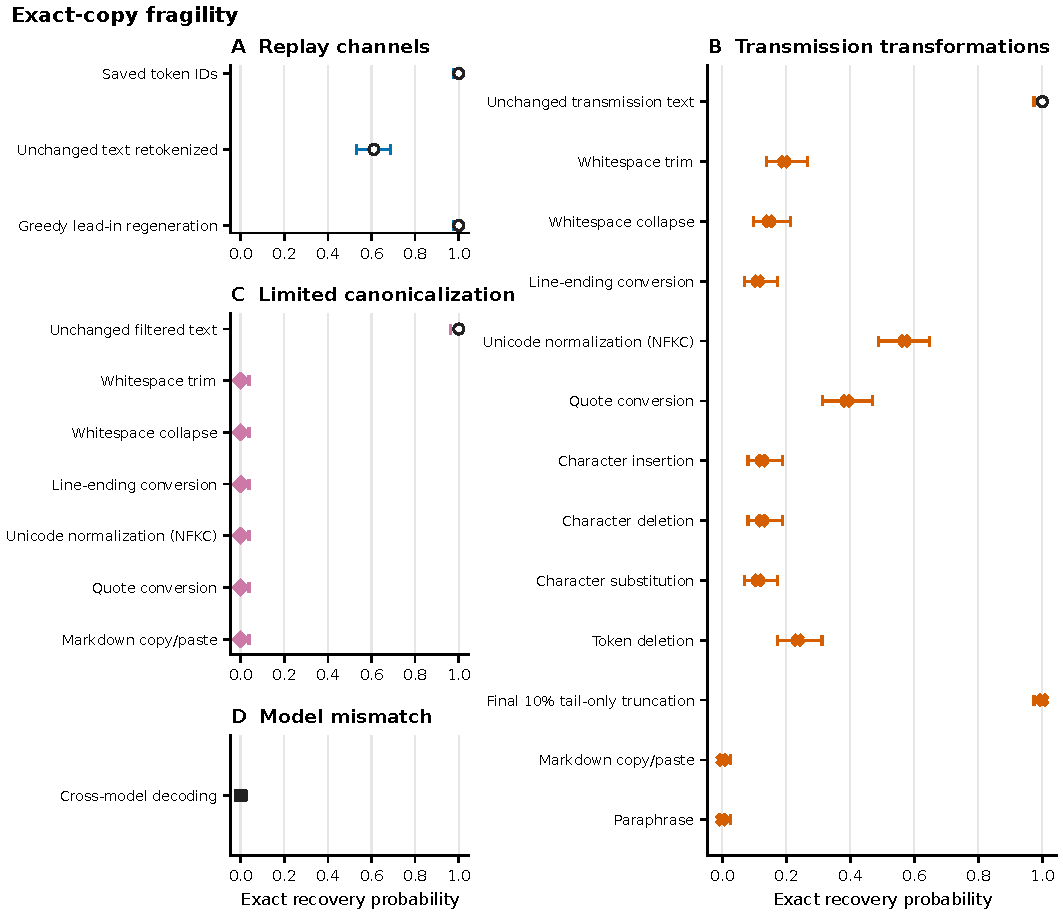
\includegraphics[width=\textwidth]{figures/robustness_recovery.pdf}
\caption{\label{fig:s1}\textbf{Complete recovery matrix and failure diagnostics.} The upper panels distinguish saved-token, visible-text, transformed-text, limited canonicalization, and cross-model replay. Intervals use source-cover Wilson calculations rather than treating two cross-model decoders as independent covers. The lower panels summarize first-divergence categories. Those categories identify the first recorded mismatch and are descriptive, not causal proof. Unavailable Mistral limited-mitigation cells are excluded rather than counted as failures.}
\end{figure}

\setlength{\tabcolsep}{3pt}
\begin{longtable}{L{0.20\textwidth}L{0.22\textwidth}r r L{0.18\textwidth}}
\caption{\label{tab:robustness}Complete principal robustness recovery table.}\\
\toprule
Family/replay & Condition & Success & Total & Wilson 95\% CI \\
\midrule
\endfirsthead
\toprule
Family/replay & Condition & Success & Total & Wilson 95\% CI \\
\midrule
\endhead
Replay: saved IDs & Unmodified & 144 & 144 & [0.974016, 1.000000] \\
Replay: detokenize/retokenize & Unmodified & 88 & 144 & [0.529589, 0.686859] \\
Replay: greedy lead-in regeneration & Unmodified & 144 & 144 & [0.974016, 1.000000] \\
Raw transmission & Unmodified & 144 & 144 & [0.974016, 1.000000] \\
Raw transmission & Final 10\% tail-only truncation & 144 & 144 & [0.974016, 1.000000] \\
Raw transmission & Unicode NFKC & 82 & 144 & [0.487804, 0.647476] \\
Raw transmission & Quote conversion & 56 & 144 & [0.313141, 0.470411] \\
Raw transmission & Token deletion & 34 & 144 & [0.174168, 0.311768] \\
Raw transmission & Whitespace trim & 28 & 144 & [0.138095, 0.266672] \\
Raw transmission & Whitespace collapse & 21 & 144 & [0.097405, 0.212667] \\
Raw transmission & Character deletion & 18 & 144 & [0.080551, 0.188937] \\
Raw transmission & Character insertion & 18 & 144 & [0.080551, 0.188937] \\
Raw transmission & Character substitution & 16 & 144 & [0.069559, 0.172872] \\
Raw transmission & LF-to-CRLF line endings & 16 & 144 & [0.069559, 0.172872] \\
Raw transmission & Markdown blockquote copy/paste & 0 & 144 & [0.000000, 0.025984] \\
Raw transmission & Deterministic paraphrase & 0 & 144 & [0.000000, 0.025984] \\
Cross-model retokenized & Unmodified, two alternate decoders & 0 & 288 outcomes/144 covers & source-cover CI [0.000000, 0.025984] \\
Limited canonicalization & Unmodified & 96 & 96 & [0.961524, 1.000000] \\
Limited canonicalization & Each of six available transformed cells & 0 & 96 per cell & [0.000000, 0.038476] \\
\bottomrule
\end{longtable}

The limited canonicalization cells covered line endings, markdown copy/paste, quote conversion, NFKC, whitespace collapse, and whitespace trim. Each had 96 observations and 48 unavailable Mistral source conditions. The all-zero transformed results do not support a mitigation claim.

\begin{table}[H]
\centering
\small
\begin{tabularx}{\textwidth}{L{0.21\textwidth}L{0.18\textwidth}Y Y}
\toprule
Requested class & Coverage & Frozen proxy & Boundary \\
\midrule
Whitespace changes & Direct & Trim, collapse, line endings & Separate conditions; not a pooled estimand \\
Leading/trailing whitespace & Direct & Trim & Addition was not tested \\
Unicode normalization & Direct & NFKC & Other forms untested \\
Quotation marks & Direct & Straight-to-smart conversion & Reverse/locale-specific forms untested \\
Copy/paste & Direct & Fixed markdown blockquote pipeline & Not an application/OS survey \\
Line wrapping & Partial & LF-to-CRLF proxy & No visual reflow/insertion test \\
Markdown/email quoting & Partial & Markdown blockquote & No client headers, nesting, or reflow \\
Sentence boundaries & Partial & Broad paraphrase & Boundary edits not isolated \\
Punctuation changes & Untested & None & Alphanumeric substitution is not a punctuation test \\
Arbitrary prefix/suffix & Untested & None & Blockquote markup is not general insertion \\
Case conversion & Untested & None & No estimate available \\
\bottomrule
\end{tabularx}
\caption{\label{tab:coverage}Perturbation-coverage inventory: five directly tested, three partially represented, and three untested requested classes.}
\end{table}

Failure summaries classify detokenization/retokenization divergence, whitespace/markup tokenization divergence, quotation divergence, Unicode normalization divergence, content-edit divergence, semantic rewrite divergence, and model/tokenizer identity mismatch. For example, a mismatch can appear at the first forced position because a transformed prefix changes the context, even when later visible words are unchanged. The recorded first-difference position, 'rank-out-of-bound' flag, and token/rank lengths are useful localization evidence, but they cannot distinguish all interacting causes.

\section*{Supplementary Note S5: Automated readability and model-based quality}\label{si:s5}

The computational stimulus design selected 504 rows balanced over seven conditions (72 per condition) and over all 18 prompt templates. Selection and randomization metadata were frozen in the retained manifest. Metrics were computed on visible strings. Flesch Reading Ease is a syllable/sentence surface heuristic. Surface-flag counts search declared formatting and artifact patterns. TF-IDF cosine similarity measures lexical prompt overlap. None of these quantities records a reader's judgment.

\begin{figure}[H]
\centering
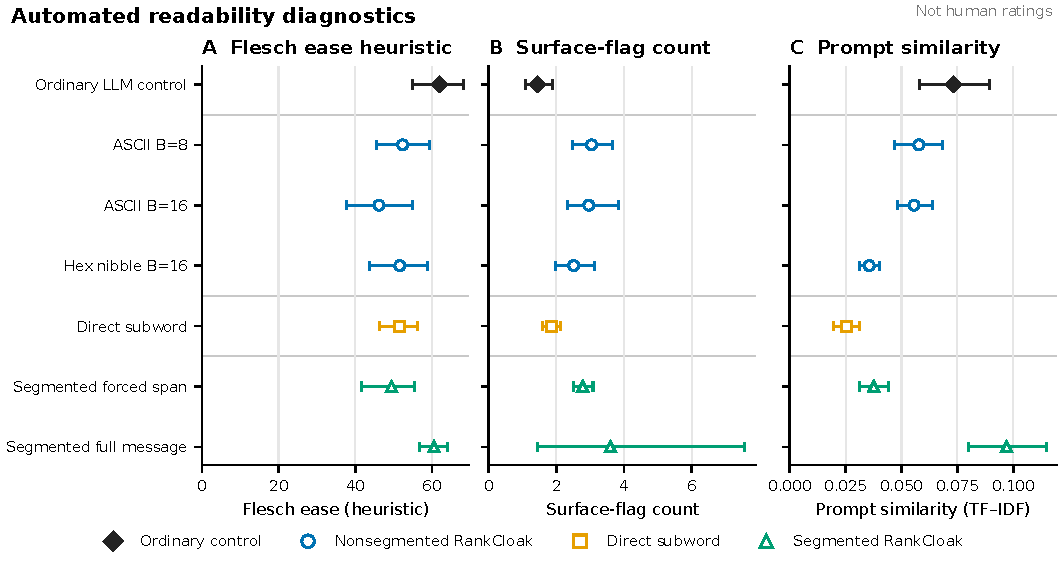
\includegraphics[width=\textwidth]{figures/automated_readability.pdf}
\caption{\label{fig:readability-full}\textbf{Automated readability diagnostics.} Flesch Reading Ease and related surface diagnostics are summarized over 504 balanced computational stimuli, with uncertainty resampled over prompt templates. Segmented full messages include payload-bearing forced spans and non-payload natural tails. These measures are automated surface properties, not human ratings, evidence of human-perceived naturalness, or substitutes for a participant study; no participant was recruited and no rating was collected.}
\end{figure}

\begin{table}[H]
\centering
\small
\begin{tabularx}{\textwidth}{L{0.30\textwidth}r L{0.25\textwidth}Y}
\toprule
Condition & Mean Flesch & Prompt-template bootstrap 95\% CI & Interpretation \\
\midrule
Ordinary control & 61.940597 & [54.897042, 68.143167] & Automated control reference \\
Segmented full message & 60.551834 & [56.873661, 64.135677] & Forced spans plus non-payload tails \\
\bottomrule
\end{tabularx}
\caption{\label{tab:readability}Principal automated readability rows. The complete figure includes all seven balanced conditions and associated surface diagnostics.}
\end{table}

Source-model quality supplied 45 protocol/model contrasts; 42 had Holm-adjusted \(p<0.05\), with estimates from -5.298565 to +2.684536. The independently held-out evaluator also supplied 45 contrasts, 42 adjusted \(p<0.05\), from -6.161972 to +3.287497. Signs differed by protocol and model, so there is no universal quality ordering. The source-cover-log-probability and held-out-evaluator mixed models were singular. Their coefficient tables remain diagnostic; no fixed-effects fallback was substituted.

The empirical capacity and quality frontier shown in Main Fig. 2 contains 4,320 trials restricted to the four payload classes on the common hexadecimal support. Three models and six protocols form 18 model and protocol cells; separate forced-span and full-message views yield 36 plotted cells. For every cell, mean token count is reported on the horizontal axis, mean source model token log probability is reported on the vertical axis, and point area represents mean automated surface-flag burden. Intervals use 2,000 payload-bootstrap resamples. Non-hexadecimal payload classes are excluded by the common-support restriction, and no lead-in condition exists in the complete primary matrix.
Forced-span metrics average only payload-bearing token positions. Full-message metrics additionally include greedy tail positions and can therefore improve as the tail becomes longer even if the forced span is unchanged. Both are reported to avoid treating tail fluency as evidence about the embedded positions.
The human-study status manifest records recruitment authorized = false, survey deployed = false, participants = 0, and ratings = 0. Planning materials are retained only to document a possible future design. They were not administered and are not reproduced here as a completed instrument. A model-name mismatch in those planning materials (Llama 3.1 versus the executed Llama 3 model) further prevents treating them as an approved executed protocol.


\section*{Supplementary Note S6: Ablations and topic effects}\label{si:s6}

\subsection*{Locked ablation extraction}

The ablation matrix paired 48 payload groups within each available model. The canonical setting was no lead-in, eight ranks per segment, the safe-text filter, and dynamic semantic stopping. Differences in Table~\ref{tab:all-ablations} are level minus canonical. These compact contrasts were extracted after outcomes were available, without fitting new models, and are classified as exploratory/post-outcome. Payload group is the pairing and 2,000-resample bootstrap unit. The printed table presents the reviewer-relevant contrasts; the complete 60-row machine-readable contrast table, including multiplicity fields and secondary outcomes, remains in the public repository.

Across the evaluated 2, 4, 8, 16, and 32 token conditions, lead-ins generally worsened likelihood, and longer lead-ins generally increased full-message length. The 32-token contrast had mean-log-probability difference -1.652327 (95\% CI, -1.749091 to -1.553103) and full-token-count difference +159.590278 (125.829861 to 191.030035). This is an adverse boundary/context result, but the paired contrast is not a causal decomposition. Segment-size changes altered efficiency and cover length: moving from 8 to 32 ranks increased effective rate by 1.231461 bits per full token (1.073116 to 1.388188) and decreased full-message length by 174.500000 tokens (-208.405035 to -140.573264). Forced-token count is codec-determined and unchanged; the length difference arises from fewer segment tails.

Removing the filter changed mean log probability by -0.001797 (-0.037738 to 0.035394) and effective rate by -0.062969 (-0.134265 to 0.007651); both selected intervals include zero. The Mistral roundtrip-stable-filter condition was unavailable for 48 work units, so the stable-filter zero rows use two models, whereas the no-filter comparison uses three. These contrasts do not establish a filter benefit.

Relative to dynamic stopping, no tail increased effective rate by 3.171551 bits per full token and reduced full-message length by 254.951389 tokens; removing non-payload text cannot be interpreted as a cover-quality improvement. The fixed sentence-tail policy of 20 to 60 tokens reduced full-message length by 65.708333 tokens. Dynamic stopping checks a frozen sentence-boundary/length predicate and then applies an emergency cap; it is not a reader judgment.

\begin{figure}[H]
\centering
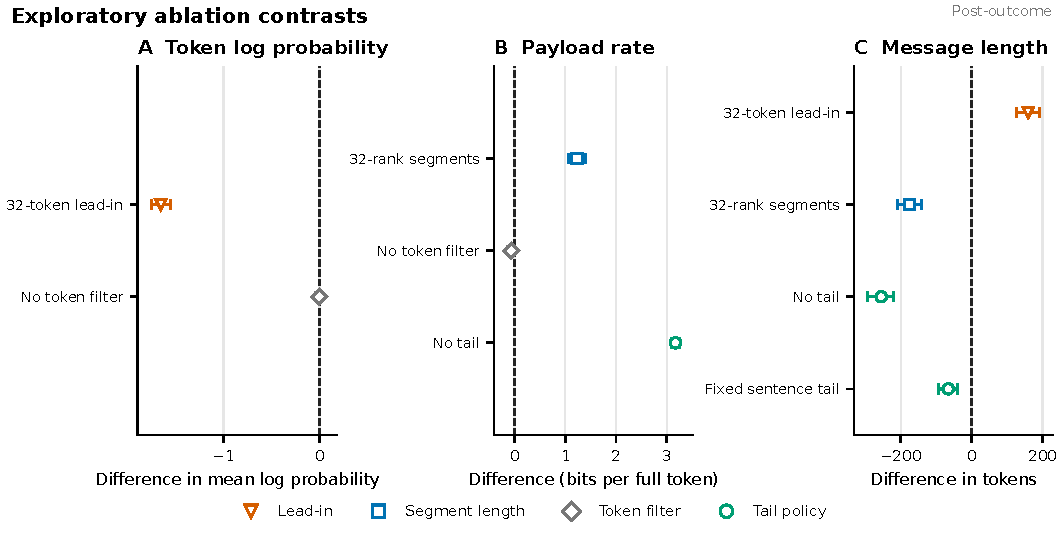
\includegraphics[width=\textwidth]{figures/ablation_summary.pdf}
\caption{\label{fig:ablation-full}\textbf{Ablation summary.} Selected paired level-minus-canonical estimates are shown with payload-bootstrap 95\% confidence intervals. Rows are exploratory/post-outcome evidence extraction from retained outputs. The Mistral roundtrip-stable-filter cell is unavailable for 48 work units; unavailable is not an execution failure. No-tail rate gains primarily reflect deletion of non-payload tokens and are not quality evidence.}
\end{figure}

\begin{table}[H]
\centering
\footnotesize
\setlength{\tabcolsep}{2.5pt}
\begin{tabularx}{\textwidth}{L{0.17\textwidth}L{0.19\textwidth}L{0.19\textwidth}L{0.19\textwidth}Y}
\toprule
Factor and level & \(\Delta\) mean log probability (95\% CI) & \(\Delta\) full tokens (95\% CI) & \(\Delta\) bits/full token (95\% CI) & Interpretation or availability \\
\midrule
Lead-in: 2 tokens & \shortstack[l]{-0.575880\\{[-0.667347, -0.491716]}} & \shortstack[l]{+13.534722\\{[-21.431424, 50.179861]}} & \shortstack[l]{-0.063224\\{[-0.157433, 0.024628]}} & Likelihood lower; length and rate intervals include zero \\
Lead-in: 4 tokens & \shortstack[l]{-0.788830\\{[-0.883630, -0.694343]}} & \shortstack[l]{+0.520833\\{[-36.346181, 35.365104]}} & \shortstack[l]{-0.051850\\{[-0.130954, 0.029064]}} & Likelihood lower; length and rate intervals include zero \\
Lead-in: 8 tokens & \shortstack[l]{-1.041886\\{[-1.115991, -0.961546]}} & \shortstack[l]{+56.750000\\{[25.909201, 87.697396]}} & \shortstack[l]{-0.179845\\{[-0.262452, -0.101276]}} & Lower likelihood, longer cover, lower rate \\
Lead-in: 16 tokens & \shortstack[l]{-1.367867\\{[-1.450430, -1.285953]}} & \shortstack[l]{+124.645833\\{[85.268229, 164.115799]}} & \shortstack[l]{-0.299132\\{[-0.379449, -0.216430]}} & Lower likelihood, longer cover, lower rate \\
Lead-in: 32 tokens & \shortstack[l]{-1.652327\\{[-1.749091, -1.553103]}} & \shortstack[l]{+159.590278\\{[125.829861, 191.030035]}} & \shortstack[l]{-0.388736\\{[-0.469659, -0.312450]}} & Largest adverse lead-in contrast \\
\addlinespace
Segment size: 4 ranks & \shortstack[l]{+0.116065\\{[0.045376, 0.192279]}} & \shortstack[l]{+212.527778\\{[172.067535, 253.639236]}} & \shortstack[l]{-0.373965\\{[-0.451966, -0.300845]}} & More segment tails; longer cover and lower rate \\
Segment size: 16 ranks & \shortstack[l]{+0.064803\\{[-0.000267, 0.131660]}} & \shortstack[l]{-104.694444\\{[-135.813021, -74.589410]}} & \shortstack[l]{+0.524216\\{[0.418241, 0.640763]}} & Fewer tails; shorter cover and higher rate \\
Segment size: 32 ranks & \shortstack[l]{+0.152306\\{[0.076589, 0.230426]}} & \shortstack[l]{-174.500000\\{[-208.405035, -140.573264]}} & \shortstack[l]{+1.231461\\{[1.073116, 1.388188]}} & Fewer tails; shortest selected cover contrast \\
\addlinespace
No filter & \shortstack[l]{-0.001797\\{[-0.037738, 0.035394]}} & \shortstack[l]{+30.090278\\{[1.998264, 59.432986]}} & \shortstack[l]{-0.062969\\{[-0.134265, 0.007651]}} & No clear likelihood or rate benefit \\
Stable filter & \shortstack[l]{0.000000\\{[0.000000, 0.000000]}} & \shortstack[l]{0.000000\\{[0.000000, 0.000000]}} & \shortstack[l]{0.000000\\{[0.000000, 0.000000]}} & Two-model invariant; Mistral unavailable, not failed \\
\addlinespace
No tail & \shortstack[l]{0.000000\\{[0.000000, 0.000000]}} & \shortstack[l]{-254.951389\\{[-292.821007, -219.249479]}} & \shortstack[l]{+3.171551\\{[3.094005, 3.244380]}} & Mechanical deletion of non-payload tokens \\
Fixed sentence tail & \shortstack[l]{0.000000\\{[0.000000, 0.000000]}} & \shortstack[l]{-65.708333\\{[-92.590451, -40.372917]}} & \shortstack[l]{-0.037921\\{[-0.113898, 0.033508]}} & Shorter than dynamic; rate interval includes zero \\
\bottomrule
\end{tabularx}
\caption{\label{tab:all-ablations}\textbf{Reviewer-relevant ablation contrasts.} Differences are level minus the canonical setting (no lead-in, eight ranks per segment, safe-text filter, and dynamic tail). Estimates pool three available models and 48 paired payloads per model except the stable-filter row, which contains two models because the 48-unit Mistral condition was unavailable. Intervals are payload-bootstrap 95\% intervals. Mean log probability is evaluated on payload-bearing forced positions; zero tail-policy differences arise because tail choice does not change those positions. All rows are exploratory/post-outcome.}
\end{table}

\subsection*{Prompt-topic contrasts}

The topic extraction compares the multi-topic and single-topic segmented schedules within model. Artifact counts are ratios on the response scale so the remaining estimates are multi-topic minus single-topic contrasts on their reported model scales. One of 15 rows excluded the null: the Llama expected artifact-count ratio was 1.276361 (95\% CI, 1.114743 to 1.461409; Holm-adjusted \(p=0.003294\)). Every other Holm-adjusted value was at least 0.396248. This locked extraction is exploratory and post-outcome where it supports neither a general topic advantage nor a new confirmatory hypothesis.

A separate exploratory subgroup display defines tail gain as full-message mean token log probability minus forced-span mean token log probability. It contains 8,280 paired segments from 1,440 segmented trials across three models, six prompt categories, and single-topic and multi-topic schedules, giving 36 displayed groups. Every group contains 230 segments, and all 36 group means were positive, ranging from +2.825721 to +3.652576. The numbers of independent payload clusters differ by schedule, 40 for single-topic and 190 for multi-topic. Uncertainty uses 2,000-resample payload-cluster bootstrapping stratified by payload class. This subgroup estimand is not equivalent to the adjusted single-topic versus multi-topic mixed-model contrast where the adjusted source-quality contrasts ranged from -0.02214 to +0.01881 and had Holm-adjusted \(p=1.0\) for all three models.

\begin{figure}[H]
\centering
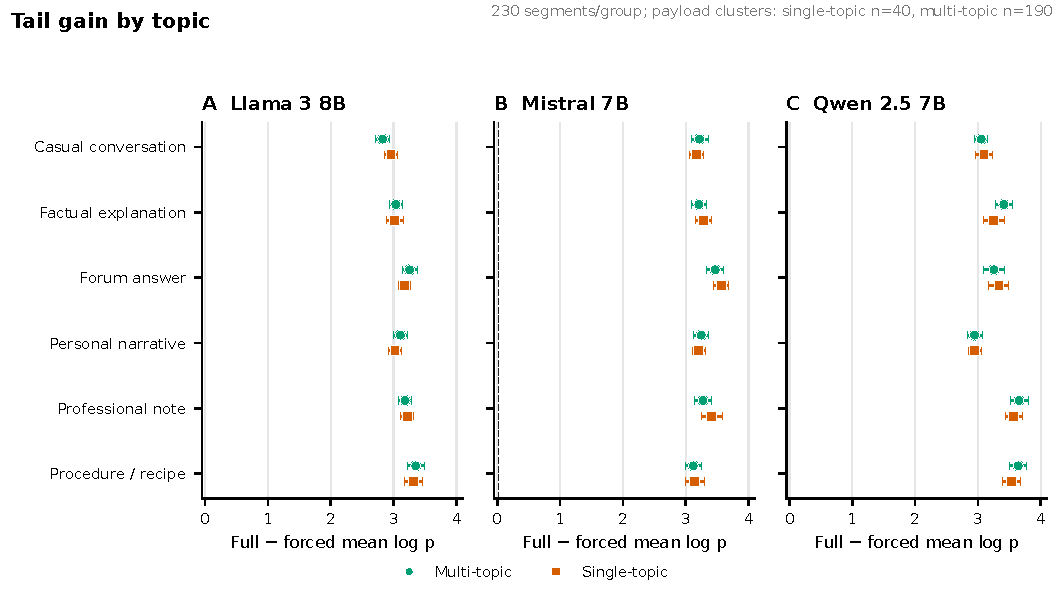
\includegraphics[width=\textwidth]{figures/tail_gain_by_prompt_category.pdf}
\caption{\label{fig:tail-gain}\textbf{Exploratory tail gain by prompt category.} Tail gain is full-message mean token log probability minus forced-span mean token log probability. The 8,280 paired segments arise from 1,440 segmented trials across three models, six prompt categories, and two topic schedules, yielding 36 displayed groups of 230 segments each. All group means are positive and range from +2.825721 to +3.652576. Uncertainty uses 2,000-resample payload-cluster bootstrapping stratified by payload class; independent payload-cluster counts are 40 for single-topic groups and 190 for multi-topic groups. This exploratory subgroup estimand is not the adjusted schedule contrast: adjusted source-quality contrasts range from -0.02214 to +0.01881, with Holm-adjusted \(p=1.0\) for all three models.}
\end{figure}

\begin{longtable}{L{0.34\textwidth}L{0.13\textwidth}r L{0.22\textwidth}r}
\caption{\label{tab:all-topic}All 15 prompt-topic contrasts.}\\
\toprule
Outcome & Model & Estimate & 95\% CI & \(p_{\rm Holm}\) \\
\midrule
\endfirsthead
\toprule
Outcome & Model & Estimate & 95\% CI & \(p_{\rm Holm}\) \\
\midrule
\endhead
Primary artifact count & Llama & 1.276361 & [1.114743, 1.461409] & 0.00329358 \\
Primary artifact count & Mistral & 1.015189 & [0.848773, 1.214233] & 1 \\
Primary artifact count & Qwen & 0.957147 & [0.781516, 1.172247] & 1 \\
Source-model log probability & Llama & -0.022140 & [-0.118718, 0.074439] & 1 \\
Source-model log probability & Mistral & 0.016347 & [-0.080231, 0.112925] & 1 \\
Source-model log probability & Qwen & 0.018813 & [-0.077766, 0.115391] & 1 \\
Effective artifact rate & Llama & 0.012473 & [-0.075124, 0.100070] & 1 \\
Effective artifact rate & Mistral & 0.006792 & [-0.080805, 0.094389] & 1 \\
Effective artifact rate & Qwen & -0.015822 & [-0.103419, 0.071775] & 1 \\
Held-out evaluator log probability & Llama & -0.012801 & [-0.129427, 0.103825] & 1 \\
Held-out evaluator log probability & Mistral & 0.012046 & [-0.104580, 0.128671] & 1 \\
Held-out evaluator log probability & Qwen & 0.024711 & [-0.091915, 0.141336] & 1 \\
Payload throughput & Llama & 0.018304 & [-0.016147, 0.052755] & 0.595439 \\
Payload throughput & Mistral & 0.026471 & [-0.007981, 0.060922] & 0.396248 \\
Payload throughput & Qwen & -0.009378 & [-0.043829, 0.025073] & 0.595439 \\
\bottomrule
\end{longtable}

\section*{Supplementary Note S7: Historical V2 neural steganalysis and leakage sensitivity}\label{si:s7}

\subsection*{Corpus, architectures, and splits}

This note preserves the historical V2 detector benchmark for continuity and work-unit provenance; its 15,840-row splits and results are not the current detector estimates and are superseded by the strictly deduplicated V3 analysis in Supplementary Notes S11--S12. The historical corpus contains 7,920 RankCloak covers and 7,920 matched ordinary controls, grouped by 480 payloads. Payload groups, rather than rows, were assigned to train, validation, and test sets. The TextCNN-equivalent implementation lowercases and tokenizes text into a 30,000-term vocabulary, truncates or pads to 256 tokens, uses 300-dimensional learned embeddings and 100 filters at each of widths 3 and 5, applies dropout 0.5, and optimizes with Adam at learning rate 0.001. The pretrained DeBERTa-v3-base classifier uses maximum length 256, learning rate \(2\times10^{-5}\), weight decay 0.01, and three epochs.
For each architecture, the frozen design comprises one matched split, 18 held-out-template splits, three leave-one-model splits, and six leave-one-codec splits. Thus 28 fits per architecture and 56/56 fits overall completed, producing 55,440 prediction rows. No row-level reassignment was used to improve performance.

For this historical benchmark, the reported endpoints were ROC-AUC and balanced accuracy. Precision, Brier score, and true-positive rate at false-positive rate at most 1\% were supplementary/exploratory post-freeze measures. All confidence intervals for an individual split use 2,000 payload-group bootstrap resamples. Ranges across heterogeneous held-out splits are descriptive minima and maxima, not confidence intervals. Every historical split-level estimate and interval remains in the machine-readable supplementary CSV (\path{supplementary_tables/detector_split_metrics.csv}).

\begin{figure}[H]
\centering
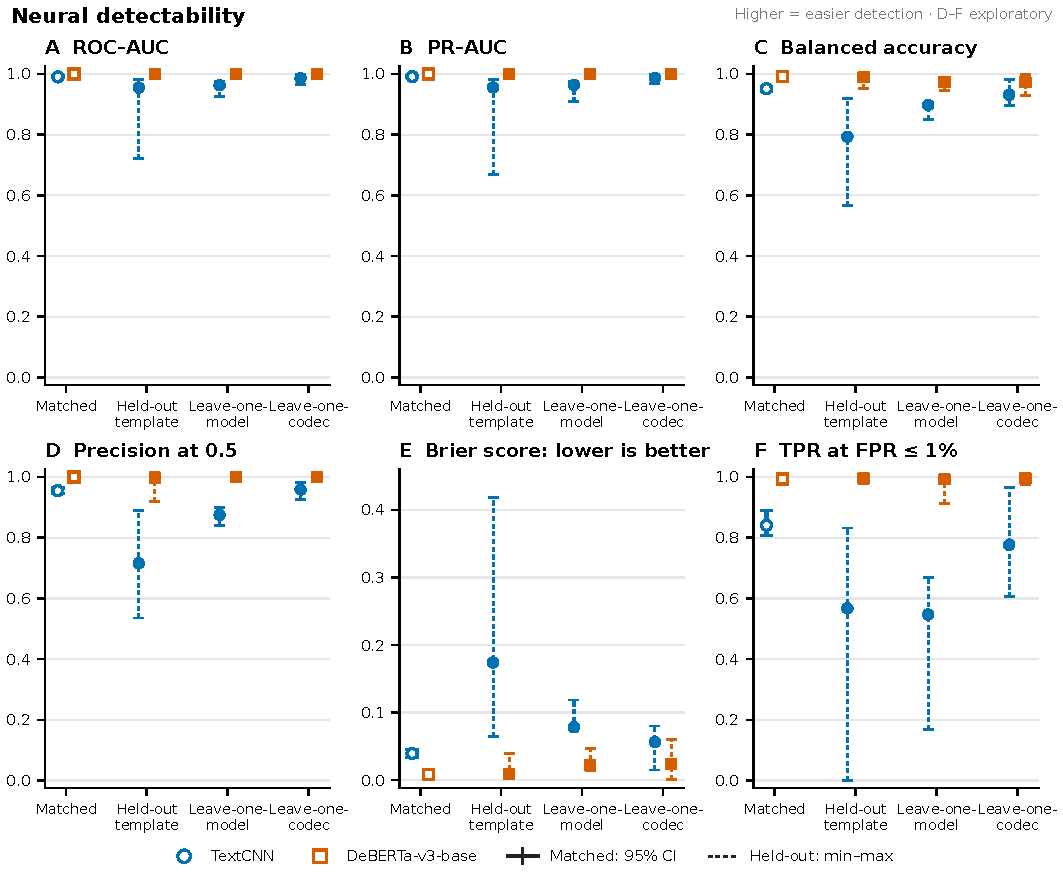
\includegraphics[width=\textwidth]{figures/neural_detector_performance.pdf}
\caption{\label{fig:detector-full}\textbf{Historical V2 neural-detector evaluation.} The six panels preserve the earlier frozen endpoints and supplementary exploratory metrics; current strictly deduplicated estimates are in Supplementary Note S12. Matched error bars are payload-group bootstrap 95\% confidence intervals. Held-out regime bars span the minimum and maximum across prespecified splits and are not confidence intervals. Lower Brier scores are better; high values in the other panels indicate stronger distinguishability and therefore weaker concealment.}
\end{figure}

\begin{table}[H]
\centering
\small
\begin{tabularx}{\textwidth}{L{0.24\textwidth}L{0.17\textwidth}r L{0.25\textwidth}Y}
\toprule
Architecture & Matched metric & Estimate & Payload-bootstrap 95\% CI & Status \\
\midrule
TextCNN-equivalent & ROC-AUC & 0.990190 & [0.987740, 0.992682] & Historical V2 frozen \\
TextCNN-equivalent & Balanced accuracy & 0.951010 & [0.943456, 0.958466] & Historical V2 frozen \\
TextCNN-equivalent & Precision & 0.954684 & [0.945891, 0.963421] & Supplementary exploratory \\
TextCNN-equivalent & Brier score & 0.039320 & [0.033497, 0.045453] & Supplementary exploratory \\
TextCNN-equivalent & TPR at FPR \(\leq1\%\) & 0.840909 & [0.806517, 0.889752] & Supplementary exploratory \\
DeBERTa-v3-base & ROC-AUC & 0.999834 & [0.999696, 0.999939] & Historical V2 frozen \\
DeBERTa-v3-base & Balanced accuracy & 0.991919 & [0.987654, 0.995665] & Historical V2 frozen \\
DeBERTa-v3-base & Precision & 0.999487 & [0.998393, 1.000000] & Supplementary exploratory \\
DeBERTa-v3-base & Brier score & 0.007895 & [0.004432, 0.011787] & Supplementary exploratory \\
DeBERTa-v3-base & TPR at FPR \(\leq1\%\) & 0.993434 & [0.988724, 0.998387] & Supplementary exploratory \\
\bottomrule
\end{tabularx}
\caption{\label{tab:detector-matched}Historical V2 matched detector endpoints, superseded for current claims by Supplementary Note S12. Higher ROC-AUC, balanced accuracy, precision, and low-FPR sensitivity are adverse for concealment; lower Brier score indicates better detector calibration.}
\end{table}

\begin{table}[H]
\centering
\small
\begin{tabularx}{\textwidth}{L{0.22\textwidth}L{0.19\textwidth}L{0.22\textwidth}Y}
\toprule
Architecture & Regime (split count) & ROC-AUC range & Balanced-accuracy range \\
\midrule
TextCNN-equivalent & Held-out template (18) & [0.720421, 0.981705] & [0.565909, 0.919318] \\
TextCNN-equivalent & Leave one model (3) & [0.925623, 0.973650] & [0.850758, 0.883333] \\
TextCNN-equivalent & Leave one codec (6) & [0.966532, 0.998634] & [0.895833, 0.980556] \\
DeBERTa-v3-base & Held-out template (18) & [0.996291, 0.999979] & [0.952273, 0.995455] \\
DeBERTa-v3-base & Leave one model (3) & [0.996772, 0.999979] & [0.945455, 0.970455] \\
DeBERTa-v3-base & Leave one codec (6) & [0.997917, 1.000000] & [0.927778, 0.998611] \\
\bottomrule
\end{tabularx}
\caption{\label{tab:detector-ranges}Historical V2 ranges across heterogeneous frozen held-out splits. These ranges are not pooled confidence intervals; current leave-one-family-out results are in Supplementary Note S12.}
\end{table}

\subsection*{Leakage, exclusion sensitivity, repeatability, and cost}

In the historical V2 benchmark, exact train/test visible-text identity and exact tokenizer-sequence identity checks passed in all 28 frozen split definitions. A separate normalized character \(n\)-gram diagnostic found 53 train/test near-duplicate pairs, of which 44 crossed payload groups, affecting 16 splits. Excluding affected test payload groups without retraining changed ROC-AUC from -0.001925 to +0.004568 for TextCNN-equivalent and from -0.000038 to +0.000166 for DeBERTa-v3-base. Because that sensitivity did not rebuild training data, it motivated and is superseded by the pre-feature component construction and zero-linkage audit in Supplementary Note S11.

Fixed-seed reruns on the same CUDA device produced exact metric equality for both architectures. This is evidence of same-device repeatability only. CPU neural training was infeasible in the retained run and no CPU result was substituted; the study makes no CPU/GPU equivalence claim. The representative CUDA benchmark recorded TextCNN wall/training times 91.358113/9.497936 seconds and peak allocated VRAM 306,247,680 bytes; DeBERTa values were 1,536.660910/1,425.063414 seconds and 6,380,851,200 bytes.

\section*{Supplementary Note S8: Capacity and quality theory}\label{si:s8}

The main Methods defines bounded forced length, nominal and effective rates, full-message overhead, and the same-context probability bound. This note gives finite-code consequences, proof conditions, and the retained-field audit without repeating those central equations.

\subsection*{Finite code space and exact inversion}

Let \(H\), \(B\), and \(n_B\) have the meanings in Main Eq.~(14). The unused capacity of the smallest fixed-length rank word is described by
\[
\sigma_B=n_B\log_2B-H,\qquad
\eta_B=\frac{2^H}{B^{n_B}}=2^{-\sigma_B},\qquad
u_B=1-\eta_B .
\]
Here \(\sigma_B\) is code-space slack in bits, \(\eta_B\) is utilization, and \(u_B\) is the unused codeword fraction. For a power-of-two alphabet and an integer-length bitstream, \(\sigma_B\) equals literal terminal padding bits. The byte codec records those bits explicitly; for \(B=8\), one byte is the finite example \(n_B=3\) with one terminal padding bit, while a multi-byte payload is packed as one continuous stream. Hex nibbles have zero slack when the represented source length is exactly four bits per canonical character.
The rank-bound proposition assumes that every forced history has at least \(B\) eligible candidates and that encoder and decoder reproduce the same model, token IDs, prompt context, mask, and ordering. A digit \(d\in\{0,\ldots,B-1\}\) selects the token at filtered rank \(d+1\); exact replay ranks that same saved token as \(d+1\). Serial induction over the forced span recovers the rank word, and injectivity of the codec recovers the representation. The proposition does not apply after an altered token, context, boundary, mask, or model, and it supplies no edit-correction property.

\subsection*{Segmentation and overhead decomposition}

For segment forced lengths \(s_j\), lead-in lengths \(\ell_j\), and tail lengths \(t_j\), the saved records satisfy \(\sum_js_j=n_B\). The empirically audited residual can be decomposed as
\[
D=N_{\mathrm{full}}-n_B
 =\sum_{j=1}^{J}(\ell_j+t_j)+\delta,\qquad \delta\ge0 .
\]
Thus segmentation alone preserves forced-position count, while more resets can create more opportunities for non-payload continuations. A no-tail condition raises bits per full token by shrinking the denominator. This is an arithmetic consequence and not evidence that the resulting visible text is more readable or natural.



\subsection*{Conditional likelihood gap}

The per-history ordering in Main Eq.~(16) permits a trace-level comparison with the rank-1 eligible token and, for bounded codecs, the rank-\(B\) token. In addition to \(Q_B\), the audit records
\[
\Delta_B
 = Q_B-Q_{\mathrm{greedy}}
 =\frac{1}{n_B}\sum_{i=1}^{n_B}
   \left[-\log p_M(y_i\mid h_i)+\log p_{(1)}(h_i)\right]\ge0 .
\]
The upper rank-\(B\) endpoint is evaluated only when its probability was retained under the identical filtered history. Direct subword traces have no single fixed \(B\), so that endpoint is unavailable rather than imputed. These quantities are model-scale surprisals in nats per forced token, not linguistic or participant outcomes.

\subsection*{Empirical checks and trace boundary}

The validation inventory contained 17,424 eligible retained records. Of these, 7,008 had all fields required for complete capacity, rate, and supported quality-bound checks. Across evaluable traces there were zero forced-position-count violations, zero rank/rate-bound violations, and zero supported quality-bound violations. The nine aggregate cells in the theoretical capacity panel of Supplementary Fig. S6 lay exactly on the identity between theoretical and observed forced positions. There were 2,976 positive cover-length residuals, attributable to natural tails or other counted cover extension.

The complete encoder decoder cascade proposition is not directly trace-evaluable from the saved record structure: none of the retained rows simultaneously carries every intermediate object required to replay the entire proof chain as one trace. The algebraic results are therefore conditional proofs and the retained-field checks are supporting empirical validation, not a complete end-to-end trace proof. They also do not validate human naturalness.

This theoretical validation asks whether the retained fields satisfy the declared fixed-radix identities, rate bounds, and supported same-context likelihood bound. It is distinct from the empirical capacity and quality frontier in Main Fig. 2, which compares observed representation rates and automated model/surface diagnostics on common payload support.

\begin{figure}[H]
\centering
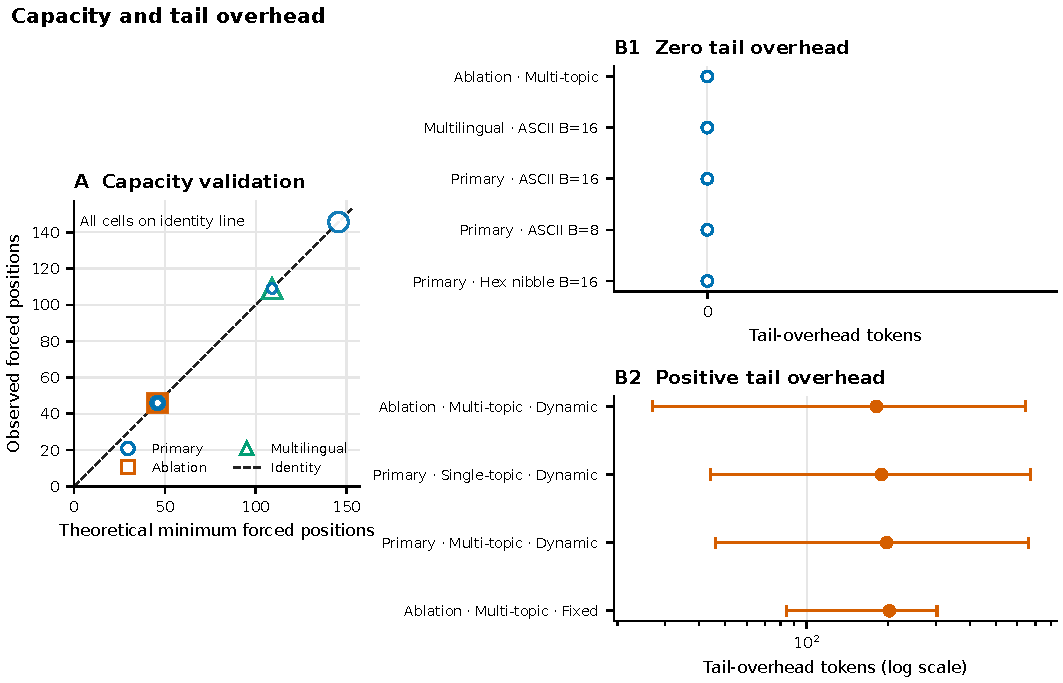
\includegraphics[width=\textwidth]{figures/capacity_tail_validation.pdf}
\caption{\label{fig:capacity-validation}\textbf{Theoretical capacity and tail validation.} Fixed-radix payload length and effective full-message rate are checked against their declared algebraic bounds, while the cover-length residual isolates tokens beyond the forced payload positions. Across 17,424 retained records, 7,008 were evaluable for the complete plotted capacity and supported quality-bound checks; no forced-position, rate-bound, or evaluated quality-bound violation occurred. Positive residuals in 2,976 records represent natural tails or other cover overhead. This validation tests retained-field identities and differs from the empirical common-support frontier in Main Fig. 2; neither analysis is evidence of human-perceived naturalness.}
\end{figure}

\begin{table}[H]
\centering
\small
\begin{tabularx}{\textwidth}{L{0.34\textwidth}r Y}
\toprule
Validation item & Result & Interpretation \\
\midrule
Eligible records & 17,424 & Broad retained validation inventory \\
Fully evaluable records & 7,008 & All required trace fields present \\
Forced-position violations & 0 & Observed count matched codec requirement \\
Rank/rate violations & 0 & Evaluated bounded-codec relations held \\
Supported quality-bound violations & 0 & Model-scale trace bound held where evaluable \\
Positive cover-length residuals & 2,976 & Tail/cover overhead, not error \\
Complete cascade traces & 0 & End-to-end proposition not directly trace-evaluable \\
\bottomrule
\end{tabularx}
\caption{\label{tab:theory-validation}Empirical capacity and traceability audit.}
\end{table}

\section*{Supplementary Note S9: Computational overhead}\label{si:s9}

Primary-stage timing used 12,144 matched payload rows across the 18 model and protocol cells in Table~\ref{tab:overhead-cells}. Intervals are 2,000-resample payload-group bootstrap intervals. Generation time is retained inclusive wrapper wall time; representation, filter setup, model generation, and supported recovery fields are reported separately in the sealed tables but are not claimed to be perfectly isolated kernel timings. Encoding wrapper time and supported decoding measurements consequently should not be summed as independent hardware primitives.

Across the 18 cells, mean inclusive generation time ranged from 1.674368 to 16.087628 seconds and payload throughput from 13.631855 to 100.851772 bits/s; effective payload rate ranged from 0.710004 to 7.322003 bits per full token. Direct-rank and hex-nibble protocols were generally faster than the byte-expanded conditions, while segmented protocols were generally slower because they repeated prompt and tail work. These retained inclusive wall-time measurements support computational accounting under the recorded hardware and harness, not universal hardware-performance claims.

\begin{figure}[H]
\centering
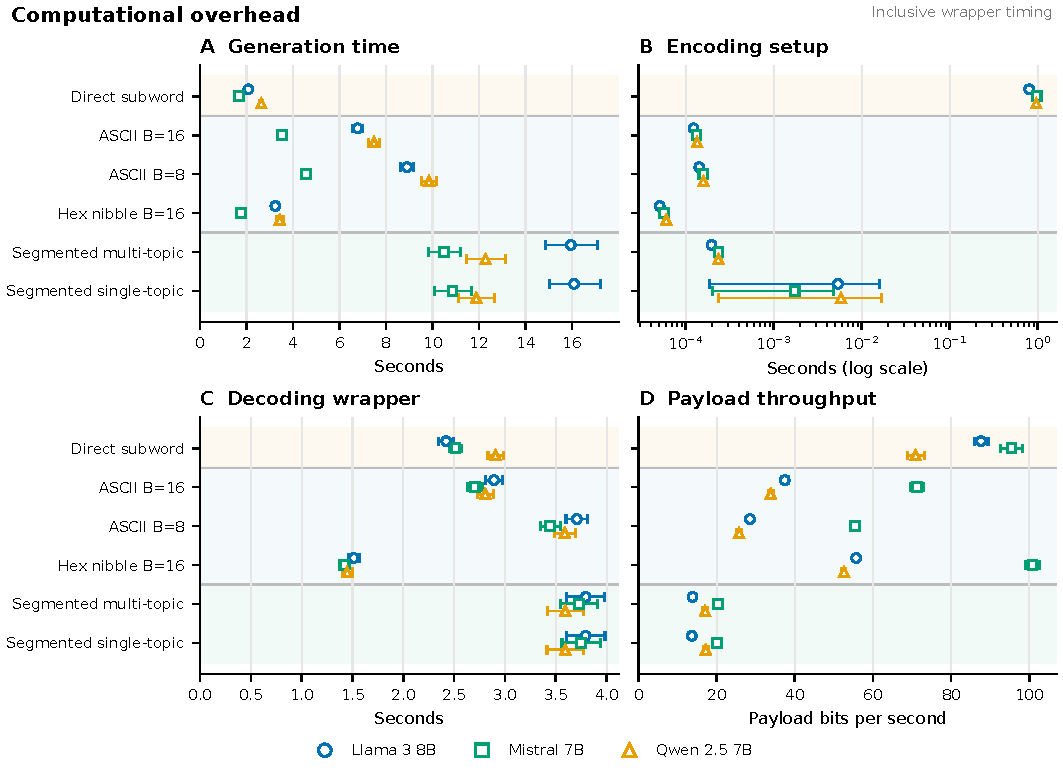
\includegraphics[width=\textwidth]{figures/computational_overhead.pdf}
\caption{\label{fig:overhead-full}\textbf{Complete computational overhead summary.} Primary model and protocol cells show payload-bootstrap summaries for inclusive generation, encoding setup, supported recovery, throughput, and effective rate. The setup panel uses a logarithmic axis because cells span several orders of magnitude. CPU time and repeated warm-up measurements were unavailable and wall time is not relabeled as CPU time.}
\end{figure}

\begin{table}[H]
\centering
\footnotesize
\setlength{\tabcolsep}{3pt}
\begin{tabularx}{\textwidth}{L{0.11\textwidth}L{0.22\textwidth}r Y Y}
\toprule
Model & Protocol & \(n\) & Mean generation time, s (95\% CI) & Mean payload throughput, bit/s (95\% CI) \\
\midrule
Llama & Direct ranks & 480 & \shortstack[l]{2.074349\\{[2.014282, 2.135219]}} & \shortstack[l]{87.658980\\{[85.892805, 89.433262]}} \\
& ASCII-16 & 480 & \shortstack[l]{6.776682\\{[6.572039, 6.982913]}} & \shortstack[l]{37.409987\\{[36.542507, 38.322129]}} \\
& ASCII-8 & 480 & \shortstack[l]{8.896445\\{[8.619910, 9.172562]}} & \shortstack[l]{28.522326\\{[27.867278, 29.213688]}} \\
& Hex-16 & 240 & \shortstack[l]{3.236699\\{[3.099398, 3.376963]}} & \shortstack[l]{55.691381\\{[55.148301, 56.225745]}} \\
& Segmented multi-topic & 240 & \shortstack[l]{15.946543\\{[14.850856, 17.084494]}} & \shortstack[l]{13.827671\\{[13.155163, 14.496873]}} \\
& Segmented single-topic & 240 & \shortstack[l]{16.087628\\{[15.017670, 17.208756]}} & \shortstack[l]{13.631855\\{[12.954794, 14.325096]}} \\
\addlinespace
Qwen & Direct ranks & 480 & \shortstack[l]{2.632108\\{[2.565827, 2.699101]}} & \shortstack[l]{70.911677\\{[68.729360, 73.171915]}} \\
& ASCII-16 & 480 & \shortstack[l]{7.480319\\{[7.242905, 7.714463]}} & \shortstack[l]{33.843456\\{[33.153343, 34.571271]}} \\
& ASCII-8 & 480 & \shortstack[l]{9.847052\\{[9.537974, 10.155572]}} & \shortstack[l]{25.724469\\{[25.198423, 26.278772]}} \\
& Hex-16 & 240 & \shortstack[l]{3.427555\\{[3.284745, 3.575041]}} & \shortstack[l]{52.584782\\{[52.074452, 53.086870]}} \\
& Segmented multi-topic & 240 & \shortstack[l]{12.276814\\{[11.449256, 13.133478]}} & \shortstack[l]{17.040206\\{[16.420206, 17.655385]}} \\
& Segmented single-topic & 240 & \shortstack[l]{11.881962\\{[11.129651, 12.646529]}} & \shortstack[l]{17.182540\\{[16.534412, 17.783251]}} \\
\addlinespace
Mistral & Direct ranks & 480 & \shortstack[l]{1.674368\\{[1.637117, 1.711610]}} & \shortstack[l]{95.454287\\{[92.689931, 98.318820]}} \\
& ASCII-16 & 480 & \shortstack[l]{3.532546\\{[3.430360, 3.637370]}} & \shortstack[l]{71.264443\\{[69.655729, 72.892828]}} \\
& ASCII-8 & 480 & \shortstack[l]{4.558496\\{[4.421249, 4.699172]}} & \shortstack[l]{55.340577\\{[54.149134, 56.561483]}} \\
& Hex-16 & 240 & \shortstack[l]{1.762009\\{[1.698523, 1.826194]}} & \shortstack[l]{100.851772\\{[99.168287, 102.554774]}} \\
& Segmented multi-topic & 240 & \shortstack[l]{10.478402\\{[9.810233, 11.196055]}} & \shortstack[l]{20.368846\\{[19.484536, 21.270824]}} \\
& Segmented single-topic & 240 & \shortstack[l]{10.858662\\{[10.074554, 11.660671]}} & \shortstack[l]{20.014386\\{[19.095928, 20.969663]}} \\
\bottomrule
\end{tabularx}
\caption{\label{tab:overhead-cells}\textbf{Inclusive generation time and payload throughput by model and protocol.} Llama denotes Meta-Llama-3-8B-Instruct, Qwen denotes Qwen2.5-7B-Instruct, and Mistral denotes Mistral-7B-Instruct-v0.3; all use the reported Q4\_K\_M configurations. Brackets contain payload-bootstrap 95\% confidence intervals.}
\end{table}

\begin{table}[H]
\centering
\small
\begin{tabularx}{\textwidth}{L{0.25\textwidth}r r r Y}
\toprule
Detector & Wall time (s) & Training time (s) & Peak allocated VRAM & Scope \\
\midrule
TextCNN-equivalent & 91.358113 & 9.497936 & 306,247,680 bytes & One fixed CUDA benchmark \\
DeBERTa-v3-base & 1,536.660910 & 1,425.063414 & 6,380,851,200 bytes & One fixed CUDA benchmark \\
\bottomrule
\end{tabularx}
\caption{\label{tab:detector-cost}Representative detector cost. CPU time, repeat warm-up measurements, and cross-device benchmarks were unavailable.}
\end{table}

\section*{Supplementary Note S10: Worked examples and claim-boundary audit}\label{si:s10}

\subsection*{Representative retained examples}

\paragraph{Payload to ranks to cover.}
A retained Llama segmented-hex trial used the public SHA-256 test-vector serialization
\begin{center}
\path{7cec7f1e68bbef4fdf066a51ccbea4377ee369e1b53219743aa386615e12d44a}.
\end{center}
The first eight encoded ranks were \([8,13,15,13,8,16,2,15]\). Under the saved prompt/model/filter state, the associated forced token IDs were \([1789,198,16,627,13617,10652,25,9842]\), detokenizing to the deliberately mechanical span
\begin{quote}
\ttfamily For\textbackslash n1.\textbackslash nExample conversation: Write
\end{quote}
The subsequent visible text
\begin{quote}
\ttfamily a friendly message to a friend about making relaxed plans for the weekend.
\end{quote}
was a natural tail. It carried no payload rank and was ignored by the decoder. Saved-token replay reproduced all nibble ranks and the serialized digest exactly. This example illustrates deterministic rank realization, not an assertion that the forced span is human-natural.

\paragraph{Visible-text retokenization failure.}
In a retained ablation trial, detokenization followed by tokenizer reapplication first diverged in segment 6, forced position 5, expected token ID 11,623 at rank 8 became observed token ID 53,992 at replay rank 2. The visible string alone therefore did not preserve the token boundary needed by the saved-token contract.

\paragraph{Transformation failure.}
For the SHA-256 example above, straight-to-smart quote conversion failed at segment 1, position 1: expected token ID 1 at rank 9, while the transformed replay observed token ID 2,118 at rank 155. The first-divergence record localizes the mismatch but does not prove that a single changed glyph alone caused every later error.

\subsection*{Claim-boundary audit}

\begin{longtable}{L{0.25\textwidth}L{0.31\textwidth}L{0.35\textwidth}}
\caption{\label{tab:claim-boundaries}Claim boundaries applied throughout the revision.}\\
\toprule
Issue & Supported statement & Prohibited or unresolved extension \\
\midrule
\endfirsthead
\toprule
Issue & Supported statement & Prohibited or unresolved extension \\
\midrule
\endhead
Exact-copy recovery & 6,480/6,480 primary serialized payloads recovered from saved token IDs under matched replay & Ordinary visible-text reliability, cross-model robustness \\
Transmission & Controlled frozen perturbations reveal severe fragility; tail-only truncation preserves recovery when only ignored tokens are removed & Broad edit robustness or general mitigation \\
Human evaluation & 504 computational stimuli have automated surface/model diagnostics & Human-perceived readability or naturalness; zero participants and ratings \\
Deployment & No operational channel or deployment traffic was tested & Practical covert communication or real-world validation \\
Detectability & Two data-adaptive text-only detectors and an exact-model-aware attacker strongly distinguish evaluated covers; high AUC is adverse & Undetectability or resistance to future detectors \\
Multilingual scope & 288/288 Spanish and 288/288 Simplified Chinese exact-copy secondary trials recovered & Broad multilingual naturalness or cross-language generalization \\
Unavailable work & 432 predeclared combinations lacked compatible retained outputs & Calling unavailable combinations experimental failures \\
Model replay & Retained outputs are bound to model/configuration manifests & Fresh local generation replay while configured GGUF files are absent \\
Detector leakage & Strict pre-feature component split has zero audited cross-partition links & Semantic paraphrases below the declared 0.95 threshold are not excluded \\
Statistical models & Reported conditional estimates retain diagnostic warnings & Treating three singular mixed-model fits as unqualified evidence; substituting an undeclared fallback \\
Exploratory analyses & Compact ablation, topic, and auxiliary detector analyses are labeled post-outcome/exploratory where applicable & Recasting them as preregistered confirmatory evidence \\
Overhead & Retained inclusive wall-time and fixed CUDA benchmark scopes are reported & CPU time, warm-up stability, CPU/GPU equivalence, or hardware-general performance \\
Theory & Conditional rank/capacity relations and retained-field checks are supported & A directly trace-evaluated full cascade or human-quality proof \\
Cryptography & The carrier can encode outputs from declared cryptographic algorithms & Cryptographic security supplied by RankCloak itself; confidentiality without an external cryptosystem \\
\bottomrule
\end{longtable}

\section*{Supplementary Note S11: Strict detector splits and human-authored secondary controls}\label{si:s11}

\subsection*{Normalization, deduplication, and partition audit}

All V3 detector corpora were deduplicated before feature extraction or tokenization. Visible text underwent Unicode NFKC normalization, case folding, Unicode-whitespace collapse, and SHA-256 hashing. If a normalized exact duplicate implicated either member of a RankCloak/control pair, the complete matched pair was removed so that class balance and pairing were preserved. Near duplicates were defined before splitting as cosine similarity at least 0.95 under L2-normalized character-boundary TF-IDF with 3--5 character \(n\)-grams and minimum document frequency two. Payload groups connected by any such edge formed immutable components.

One normalized exact-duplicate group implicated two rows in the 15,840-row source corpus. Removing that complete matched pair left 15,838 observations. The remaining audit found 52 near-duplicate pairs, including 44 that crossed payload groups. A deterministic seed-20260831 balancing procedure assigned whole connected components to train, validation, and test. The final audit found zero payload, matched-pair, normalized-text, component, or declared near-duplicate links between partitions (Table~\ref{tab:v3-dedup}). The statement of zero leakage is limited to these declared identities and thresholded edges; it cannot rule out semantic paraphrases below the threshold or guarantee real-world generalization.

\begin{table}[H]
\centering
\small
\begin{tabularx}{\textwidth}{L{0.27\textwidth}r Y}
\toprule
Audit item & Count & Interpretation \\
\midrule
Source observations & 15,840 & Balanced RankCloak and matched ordinary-model controls \\
Normalized exact groups & 1 & One complete matched pair removed, two rows total \\
Retained observations & 15,838 & 9,904 train; 2,952 validation; 2,982 test \\
Declared near-duplicate pairs & 52 & 44 cross-payload; all connected groups kept in one partition \\
Audited cross-partition links & 0 & Zero for payload, pair, normalized text, component, and declared near duplicate \\
\bottomrule
\end{tabularx}
\caption{\label{tab:v3-dedup}\textbf{Strict detector-corpus construction.} Counts are from the locked V3 deduplication audit. Zero audited leakage applies only under the stated normalization and similarity rule.}
\end{table}

\subsection*{Human-authored control selection and scope}

The secondary controls came from Databricks Dolly 15k v1.0, revision \texttt{\seqsplit{bdd27f4d94b9c1f951818a7da7fd7aeea5dbff1a}}, under CC BY-SA 3.0. Deterministic screening retained responses without automatic quality, personally identifiable information, or unsafe-content flags. The same exact and near-duplicate rules were applied within the human-authored candidates and against the primary corpus. Hungarian assignment matched candidates to RankCloak test texts within available prompt templates using relative word-count plus weighted character-count difference; relative word-count differences above 0.35 were rejected.

The pipeline selected 250 texts spanning 16 of 18 templates. It found no normalized exact duplicates, no within-human near-duplicate pairs, and no declared near-duplicate links to the primary corpus. Human labels never entered model fitting or threshold selection. The corpus is a bounded secondary computational control, not recruitment, a participant study, a user study, a human rating exercise, or proof of naturalness. Coverage is sparse or absent for several conversational, narrative, and professional templates, and detector performance can include generic machine-versus-human differences.

\begin{table}[H]
\centering
\small
\begin{tabularx}{\textwidth}{L{0.28\textwidth}r Y}
\toprule
Human-control item & Result & Scope \\
\midrule
Selected responses & 250 & Frozen test negatives from Dolly; 16 templates represented \\
Within-human exact links & 0 & Under NFKC/casefold/whitespace normalization \\
Within-human near links & 0 & Under the declared 0.95 character-\(n\)-gram rule \\
Human-to-primary near links & 0 & Same declared rule \\
Labels used for fitting/thresholds & No & Thresholds came from matched ordinary-model validation controls \\
Empirical 0.1\% FPR & Unavailable & Only 250 human negatives; at least 1,000 required \\
\bottomrule
\end{tabularx}
\caption{\label{tab:v3-human-design}Human-authored secondary-control design and audit.}
\end{table}

\section*{Supplementary Note S12: Deduplicated, unseen-family, model-aware, and low-FPR detection}\label{si:s12}

The text-only attackers reuse the fixed V1 TextCNN and pinned \path{microsoft/deberta-v3-base} revision \texttt{\seqsplit{8ccc9b6f36199bec6961081d44eb72fb3f7353f3}}. Their architectures and hyperparameters were not tuned on V3 test data. They are data-adaptive black-box attackers because they are fitted specifically to distinguish RankCloak from matched ordinary-model output. The model-aware logistic attacker instead receives saved token log probabilities from the exact generation model and uses summary surprisal features. Its L2 regularization value was chosen from 0.01, 0.1, 1, and 10 by validation ROC-AUC. Rank-only fields were excluded because ordinary-control ranks were not stored.

Matched fitting used 9,904 training and 2,952 validation observations; the test had 1,491 positives and 1,491 negatives. For each leave-one-family-out fit, the target family was absent from both training and validation, and evaluation used only its 497 positive and 497 negative observations in held test components. Table~\ref{tab:v3-detector-main} reports the adverse matched results and the range across the three genuine family holdouts.

\begin{table}[H]
\centering
\small
\setlength{\tabcolsep}{3pt}
\begin{tabularx}{\textwidth}{L{0.22\textwidth}L{0.20\textwidth}L{0.23\textwidth}Y}
\toprule
Detector & Matched ROC-AUC (95\% CI) & Matched normalized 0--1\% pAUC & Leave-one-family-out ROC-AUC range \\
\midrule
TextCNN & 0.9868 [0.9819, 0.9913] & 0.6652 & [0.9186, 0.9784] \\
DeBERTa-v3-base & 0.9994 [0.9984, 1.0000] & 0.9948 & [0.9972, 1.0000] \\
Model-aware surprisal & 0.999995 [0.999970, 1.000000] & 0.999460 & [0.999943, 1.000000] \\
\bottomrule
\end{tabularx}
\caption{\label{tab:v3-detector-main}\textbf{Detection on strictly deduplicated components.} The matched test has 1,491 observations per class. Ranges summarize three distinct held-family tests and are not pooled confidence intervals. Higher values are adverse for concealment.}
\end{table}

ROC-AUC used tie-aware empirical ranks. The normalized 0--1\% partial AUC was the exact empirical false-positive-budget step envelope divided by 0.01; no score or ROC vertex was interpolated. At target \(\alpha\), the validation threshold maximized TPR subject to no more than \(\lfloor\alpha n_{\rm neg}\rfloor\) false positives, with conservative tie breaking. The threshold was then frozen for test. A target was reported only if validation and test both contained at least \(1/\alpha\) negatives. Confidence intervals used 2,000 percentile bootstrap resamples of complete deduplication clusters.

\begin{table}[H]
\centering
\scriptsize
\setlength{\tabcolsep}{2.5pt}
\begin{tabularx}{\textwidth}{L{0.17\textwidth}L{0.14\textwidth}r r L{0.18\textwidth}L{0.18\textwidth}Y}
\toprule
Detector & Evaluation & Val.\ negatives & Test negatives & Test TPR/FPR at frozen 1\% threshold & Exact false positives & Frozen 0.1\% result \\
\midrule
TextCNN & Matched & 1,476 & 1,491 & 0.8317/0.0127 & 19/1,491 & TPR 0.4829; FPR 0.0013; 2/1,491 FP \\
DeBERTa & Matched & 1,476 & 1,491 & 0.9913/0.0007 & 1/1,491 & TPR 0.9886; FPR 0.0007; 1/1,491 FP \\
Model-aware & Matched & 1,476 & 1,491 & 0.9987/0.0020 & 3/1,491 & TPR 0.9987; FPR 0.0020; 3/1,491 FP \\
TextCNN & Held family range & 984 & 497 & TPR 0.7103--0.8330; FPR 0.0201--0.0704 & 10--35/497 & Unavailable: fewer than 1,000 negatives \\
DeBERTa & Held family range & 984 & 497 & TPR 0.9759--1.0000; FPR 0.0040--0.0563 & 2--28/497 & Unavailable: fewer than 1,000 negatives \\
Model-aware & Held family range & 984 & 497 & TPR 0.9920--1.0000; FPR 0.0000--0.0060 & 0--3/497 & Unavailable: fewer than 1,000 negatives \\
\bottomrule
\end{tabularx}
\caption{\label{tab:v3-low-fpr}\textbf{Validation-frozen low-FPR operating points.} The observed test FPR can differ from the validation target. Exact counts, rather than interpolated rates, expose calibration drift and empirical resolution.}
\end{table}

\begin{figure}[H]
\centering
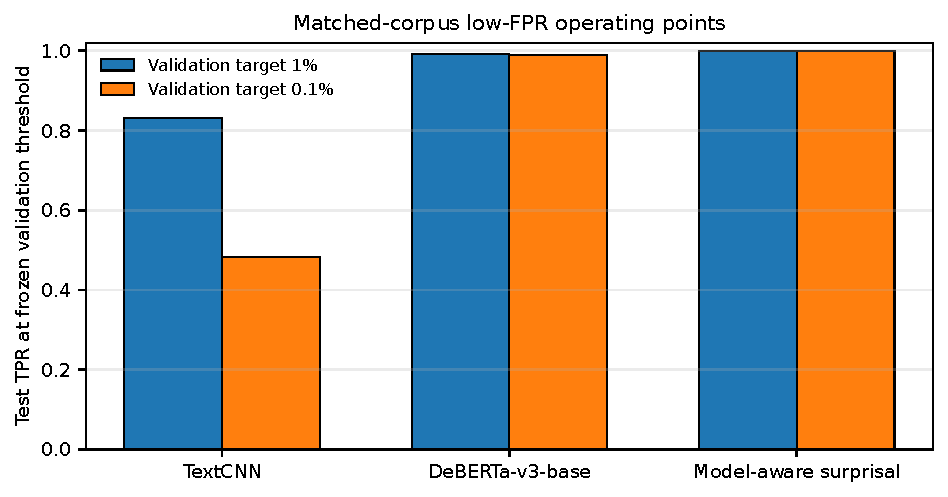
\includegraphics[width=\textwidth]{figures/detector_low_fpr.pdf}
\caption{\label{fig:v3-low-fpr}\textbf{Low-FPR detection under frozen thresholds.} Thresholds were selected on validation and applied once to test. Missing 0.1\% family-holdout results reflect insufficient negative counts, not zero sensitivity.}
\end{figure}

Against the human-authored secondary controls, TextCNN ROC-AUC was 0.7537 (95\% CI [0.7141, 0.7918]) and DeBERTa ROC-AUC was 0.9846 (95\% CI [0.9771, 0.9910]). At the thresholds selected on ordinary-model validation controls for nominal 1\% FPR, TextCNN classified 152/250 human texts as positive (FPR 0.6080; grouped-bootstrap 95\% CI [0.5469, 0.6667]) and DeBERTa classified 97/250 as positive (FPR 0.3880; CI [0.3263, 0.4466]). These high false-positive rates show domain sensitivity and do not reverse the matched-control result.

\begin{figure}[H]
\centering
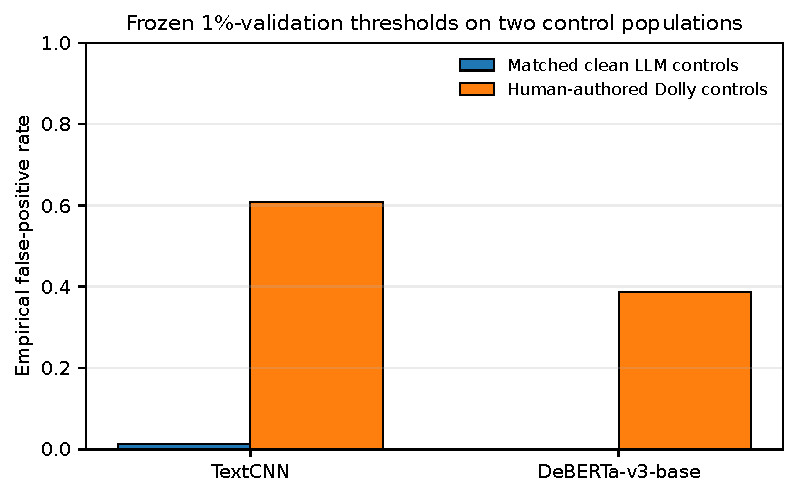
\includegraphics[width=\textwidth]{figures/human_control_false_positives.pdf}
\caption{\label{fig:v3-human-controls}\textbf{Secondary human-authored control evaluation.} Human-authored labels were not used for fitting or threshold selection. The comparison may include general machine-versus-human signal and is not a human evaluation.}
\end{figure}

The two learned detectors adapt to the observed training distribution; the likelihood-based detector represents an attacker with exact model access. Their strength makes the negative detectability conclusion more credible within the evaluated corpus, but none is a comprehensive adversarial search over all classifiers, prompts, post-processing, models, or deployment distributions.

\section*{Supplementary Note S13: Entropy-gated payload embedding}\label{si:s13}

\subsection*{Calibration and replay-consistent gate}

The entropy-gated extension was informed by Cai, Ding, and Tao\cite{Cai2025EntropyGuidedWatermarking}, but the objectives differ. Their watermarking detector decides whether text carries a mark; a RankCloak receiver must reconstruct an arbitrary payload. Selective watermark insertion therefore does not by itself establish payload capacity, recoverability, or concealment.

Six 128-position ordinary top-\(p\) traces per model used temperature 0.8, top-\(p\) 0.95, and the frozen serial sampler, yielding 768 development positions per model. Detector outcomes did not enter calibration. The median threshold defines the moderate gate and the 75th percentile defines the strict gate (Table~\ref{tab:v3-entropy-thresholds}).

\begin{table}[H]
\centering
\small
\begin{tabularx}{\textwidth}{L{0.34\textwidth}r r r}
\toprule
Model & Traces & Median threshold, bit & 75th-percentile threshold, bit \\
\midrule
Llama 3 8B Q4\_K\_M & 6 & 0.803259 & 1.705455 \\
Mistral 7B Q4\_K\_M & 6 & 0.966861 & 1.917551 \\
Qwen 2.5 7B Q4\_K\_M & 6 & 1.361919 & 2.432557 \\
\bottomrule
\end{tabularx}
\caption{\label{tab:v3-entropy-thresholds}Frozen entropy thresholds from ordinary-generation development traces.}
\end{table}

Before each embedding-span step, the encoder computed filtered next-token Shannon entropy. An eligible position consumed and forced the next payload rank. An ineligible position used ordinary top-\(p\) sampling under the same allowed-token mask and did not consume a payload rank. Replay recomputed entropy before each observed token, consumed a rank only at eligible positions, ignored observed ranks at sampled skips, and appended every observed token to context. It received no saved gate-position metadata. Gate-position agreement between encoder and replay was exact in the validation audit.

Each gate contained 120 RankCloak attempts and 120 paired length-matched ordinary controls across three model families, eight artifact classes, all 20 supported artifact/representation cells, and two templates. The ungated, moderate, and strict RankCloak conditions shared one stable seed per cell; controls used a separate shared ordinary-generation seed. Fixed-token-budget capacity was evaluated at the paired ungated span length for every attempt. Fixed-payload bits per generated token was defined only when the complete payload was embedded; completion rate and fixed-budget payload fraction are therefore separate endpoints.

\begin{table}[H]
\centering
\scriptsize
\setlength{\tabcolsep}{3pt}
\begin{tabularx}{\textwidth}{L{0.13\textwidth}r r L{0.18\textwidth}r r r Y}
\toprule
Gate & Complete & Budget failures & Capacity, bit/token & Capacity \(n\) & Budget payload fraction & Length ratio & Saved-ID/visible recovery \\
\midrule
Ungated & 120/120 & 0 & 7.4001, conditional & 120 & 1.0000 & 1.0000 & 120/120; 62/120 \\
Moderate median & 120/120 & 0 & 5.7920, conditional & 120 & 0.7518 & 1.3743 & 120/120; 65/120 \\
Strict 75th percentile & 114/120 & 6 & 4.0513, conditional & 114 & 0.4567 & 2.7615 & 114/120; 68/120 \\
\bottomrule
\end{tabularx}
\caption{\label{tab:v3-entropy-generation}\textbf{Entropy-gate generation, capacity, length, and recovery.} Capacity is fixed-payload bits per generated token conditional on completion. In particular, strict-gate capacity excludes six incomplete cases and has \(n=114\). Completion and recovery retain all 120 attempts in their denominators.}
\end{table}

Strict completion by model was 40/40 for Llama, 39/40 for Mistral, and 35/40 for Qwen. The corresponding strict conditional capacity estimates were 6.1322 (\(n=40\)), 2.9207 (\(n=39\)), and 2.9331 (\(n=35\)) bits/token. Visible-text recovery under ungated/moderate/strict conditions was 29/40, 29/40, and 34/40 for Llama; 0/40 in every Mistral condition; and 33/40, 36/40, and 34/40 for Qwen. The aggregate visible-text differences therefore do not establish a general gate benefit.

Relative to ungated output, moderate gating added a mean 20.1083 words, changed unique-word fraction by \(-0.0338\), and changed repeated-bigram fraction by \(+0.0106\). Strict gating added 103.0083 words, changed unique-word fraction by \(-0.1431\), and changed repeated-bigram fraction by \(+0.0423\). These are surface heuristics, not participant judgments. At forced payload positions, mean rank was 88.0552 for ungated and moderate gates and 89.4915 for the strict gate; mean forced-token rank pressure declined from 3.8585 to 3.4276 and 3.0308 nats. Gating changes the contexts in which payload ranks are consumed but does not change the payload-rank distribution for completed paired cells.

\begin{figure}[H]
\centering
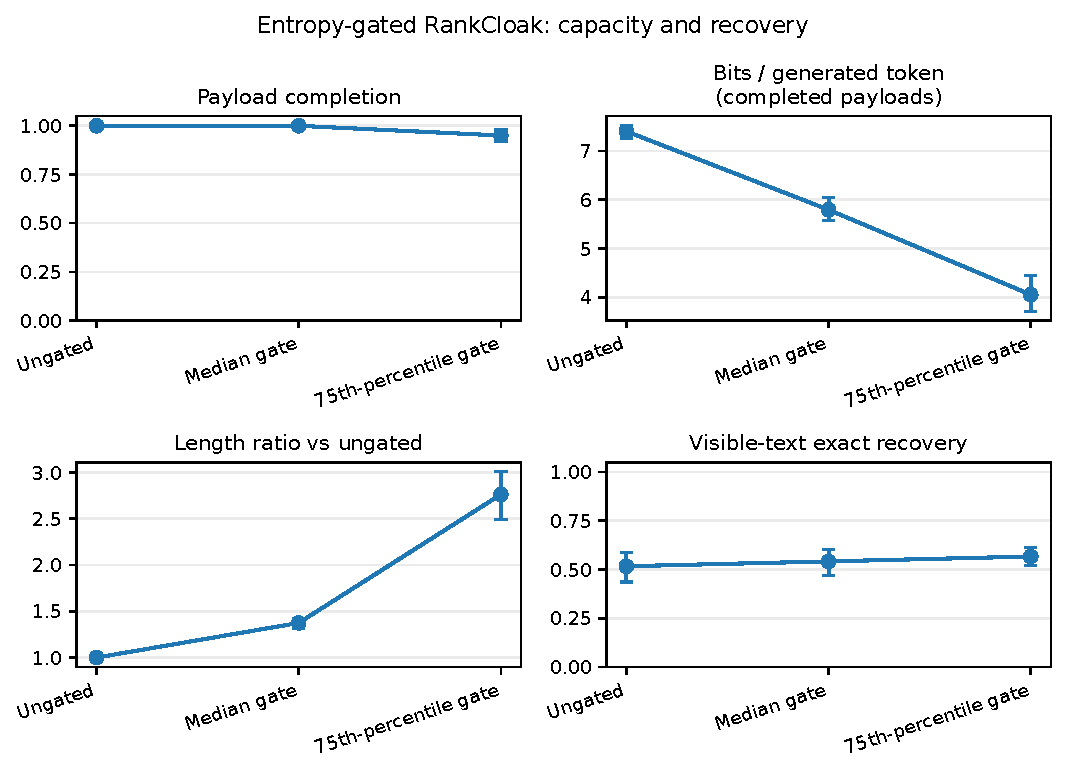
\includegraphics[width=\textwidth]{figures/entropy_gate_capacity_recovery.pdf}
\caption{\label{fig:v3-entropy-capacity}\textbf{Entropy gating, capacity, length, completion, and recovery.} Fixed-payload capacity is conditional on completion; fixed-budget payload fraction and completion retain all attempts.}
\end{figure}

The generated detector test was external to fitting. Historical train and validation rows carrying any of the 16 entropy-study payload instances were excluded, and exact/near-duplicate auditing was repeated before feature extraction. The audit retained 12,714/13,114 rows, removed 400, found zero cross-partition links, and left no condition unavailable. Gate-specific test controls numbered 117 ungated, 113 moderate, and 116 strict; none supports empirical 0.1\% resolution.

\begin{table}[H]
\centering
\scriptsize
\setlength{\tabcolsep}{2.5pt}
\begin{tabularx}{\textwidth}{L{0.18\textwidth}L{0.12\textwidth}r r r L{0.18\textwidth}Y}
\toprule
Detector & Gate & Pos./neg. & ROC-AUC & 0--1\% pAUC & TPR/FPR at frozen 1\% threshold & Exact FP \\
\midrule
TextCNN & Ungated & 117/117 & 0.9953 & 0.8536 & 0.8718/0.0085 & 1/117 \\
TextCNN & Moderate & 113/113 & 0.9825 & 0.7416 & 0.7965/0.0088 & 1/113 \\
TextCNN & Strict & 116/116 & 0.8850 & 0.4138 & 0.4310/0.0172 & 2/116 \\
DeBERTa & Ungated & 117/117 & 0.9999 & 0.9854 & 1.0000/0.0085 & 1/117 \\
DeBERTa & Moderate & 113/113 & 0.9785 & 0.6878 & 0.8496/0.0177 & 2/113 \\
DeBERTa & Strict & 116/116 & 0.8893 & 0.3484 & 0.4914/0.0259 & 3/116 \\
Model-aware & Ungated & 117/117 & 1.0000 & 1.0000 & 1.0000/0.0000 & 0/117 \\
Model-aware & Moderate & 113/113 & 0.9999 & 0.9922 & 0.9381/0.0000 & 0/113 \\
Model-aware & Strict & 116/116 & 0.9904 & 0.7845 & 0.6552/0.0000 & 0/116 \\
\bottomrule
\end{tabularx}
\caption{\label{tab:v3-entropy-detectors}\textbf{Detector behavior by entropy gate.} Thresholds are the single historical-validation-frozen nominal 1\% thresholds. Every gate has fewer than 1,000 test negatives, so empirical 0.1\% TPR is unavailable.}
\end{table}

\begin{figure}[H]
\centering
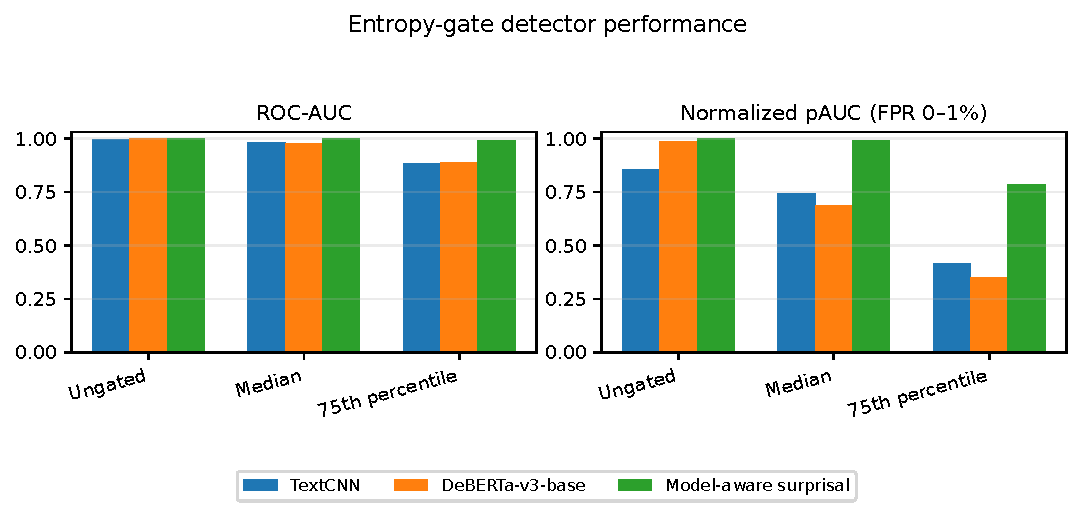
\includegraphics[width=\textwidth]{figures/entropy_gate_detector_performance.pdf}
\caption{\label{fig:v3-entropy-detectors}\textbf{Entropy-gate detector performance.} Stricter gating reduces text-only detectability in this bounded matrix but does not eliminate the strong exact-model-aware signal.}
\end{figure}

Taken together, stricter gating reduces text-only detection in the tested conditions while reducing capacity, substantially increasing length, producing six maximum-budget failures, and retaining exact-environment replay dependence. Model-aware ROC-AUC of 0.9904 under the strict gate is inconsistent with a claim of an undetectable channel.

\section*{Supplementary Note S14: Matched Q4 and Q8 quantization analysis}\label{si:s14}

\subsection*{Pairing and recovery}

The quantization analysis holds Qwen2.5-7B-Instruct revision \path{8911e8a47f92bac19d6f5c64a2e2095bd2f7d031}, its embedded tokenizer, rendered prompt, payload, codec, safe-text filter, target length, temperature, top-\(p\), llama-cpp-python 0.3.23 backend, and historical ordinary-control seed fixed. It successfully model-replayed all 1,920 historical Q4\_K\_M rows and completed all 1,920 paired Q8\_0 generations. No additional Q4 covers were generated.

Visible-text recovery for the 960 historical Q4 RankCloak covers retokenized each recorded string under the exact embedded Q4 tokenizer. The 732 exact token-ID matches reused the validated saved-ID rank trace; the other 228 cases underwent rank replay through the pinned Q4 model with the saved embedding-span boundary. This remains replay-assisted and does not recover without the exact context and span contract. Q8 visible-text recovery used the corresponding exact model path. Pairing used frozen payload, representation, and prompt identities.

\begin{table}[H]
\centering
\small
\begin{tabularx}{\textwidth}{L{0.32\textwidth}r r Y}
\toprule
Recovery item & Q4\_K\_M & Q8\_0 & Paired interpretation \\
\midrule
Saved-ID exact recovery & 960/960 & 960/960 & Perfect only under exact saved-ID replay \\
Visible-text exact recovery & 732/960 (0.7625) & 758/960 (0.7896) & Difference 0.0271; 95\% CI [-0.0073, 0.0635] \\
Visible recovery 95\% CI & [0.7344, 0.7896] & [0.7635, 0.8167] & Payload-group bootstrap, 2,000 resamples \\
Discordant outcomes & Q4 only 144 & Q8 only 170 & Exact two-sided McNemar \(p=0.1582\) \\
Concordant outcomes & Both 588 & Neither 58 & No statistically supported Q8 advantage \\
\bottomrule
\end{tabularx}
\caption{\label{tab:v3-quant-recovery}\textbf{Paired Q4 and Q8 recovery.} Rates use 960 frozen RankCloak pairs. The exact McNemar result is computed from the stored 144/170 discordant counts.}
\end{table}

\begin{figure}[H]
\centering
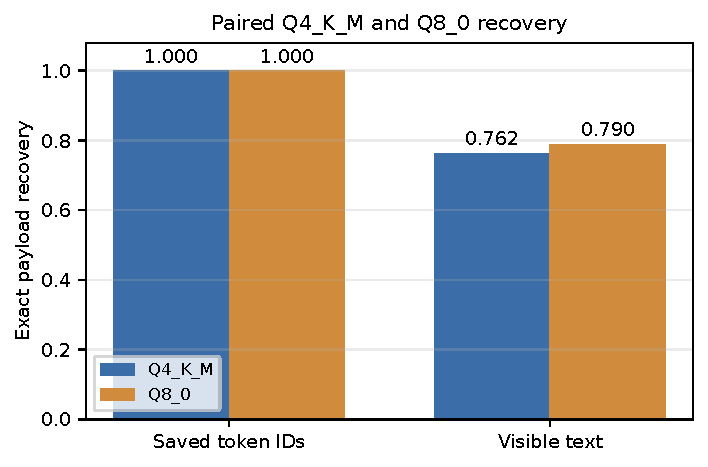
\includegraphics[width=\textwidth]{figures/matched_quantization_recovery.pdf}
\caption{\label{fig:v3-quant-recovery}\textbf{Paired saved-ID and visible-text recovery by quantization.} The grouped interval for the paired difference includes zero.}
\end{figure}

On the identical historical Q4 RankCloak token path, Q8 minus Q4 mean next-token entropy was \(-0.0154\) bits (95\% CI [-0.0187, -0.0120]); the observed-token rank changed at a mean fraction 0.4639 of positions and the greedy token changed at 0.0884. Independently generated Q4/Q8 RankCloak paths never matched exactly and had mean positionwise token match 0.0155. These differences show substantial path sensitivity; they are not evidence that either quantization is generally more recoverable.

\begin{figure}[H]
\centering
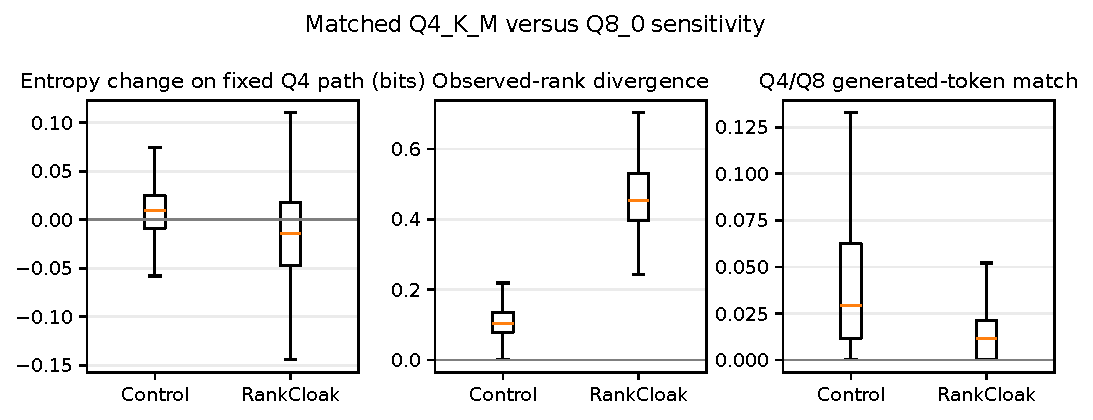
\includegraphics[width=\textwidth]{figures/matched_quantization_sensitivity.pdf}
\caption{\label{fig:v3-quant-sensitivity}\textbf{Matched quantization sensitivity.} Same-path likelihood/rank comparisons and independently generated token-path agreement are paired within one pinned Qwen revision.}
\end{figure}

\subsection*{Cross-quantization detector transfer}

Quantization detectors used the frozen payload train/validation/test assignment. Q4-to-Q8 fit and selected thresholds on Q4 before testing Q8; Q8-to-Q4 reversed the direction; the pooled fit used both quantizations in training and validation and tested only held payloads. Exact and declared near-duplicate audits preceded feature extraction and retained every row: 1,920/1,920 in each directional corpus and 3,840/3,840 pooled, with zero audited leakage.

\begin{table}[H]
\centering
\scriptsize
\setlength{\tabcolsep}{2.5pt}
\begin{tabularx}{\textwidth}{L{0.17\textwidth}L{0.14\textwidth}r r L{0.19\textwidth}Y}
\toprule
Detector & Transfer & ROC-AUC & 0--1\% pAUC & TPR/FPR at frozen 1\% threshold & Exact FP \\
\midrule
TextCNN & Q4 to Q8 & 0.9927 & 0.7539 & 0.9375/0.0365 & 7/192 \\
DeBERTa & Q4 to Q8 & 1.0000 & 1.0000 & 1.0000/0.0000 & 0/192 \\
Model-aware & Q4 to Q8 & 1.0000 & 1.0000 & 1.0000/0.0000 & 0/192 \\
TextCNN & Q8 to Q4 & 0.9944 & 0.8298 & 0.9479/0.0260 & 5/192 \\
DeBERTa & Q8 to Q4 & 1.0000 & 1.0000 & 1.0000/0.0156 & 3/192 \\
Model-aware & Q8 to Q4 & 1.0000 & 1.0000 & 0.9792/0.0000 & 0/192 \\
TextCNN & Pooled & 0.9965 & 0.8257 & 0.9609/0.0234 & 9/384 \\
DeBERTa & Pooled & 1.0000 & 1.0000 & 1.0000/0.0078 & 3/384 \\
Model-aware & Pooled & 1.0000 & 1.0000 & 0.9948/0.0000 & 0/384 \\
\bottomrule
\end{tabularx}
\caption{\label{tab:v3-cross-quant-detectors}\textbf{Cross-quantization and pooled detector behavior.} Frozen nominal thresholds can drift in test. No test has 1,000 negatives, so empirical 0.1\% results are unavailable.}
\end{table}

\begin{figure}[H]
\centering
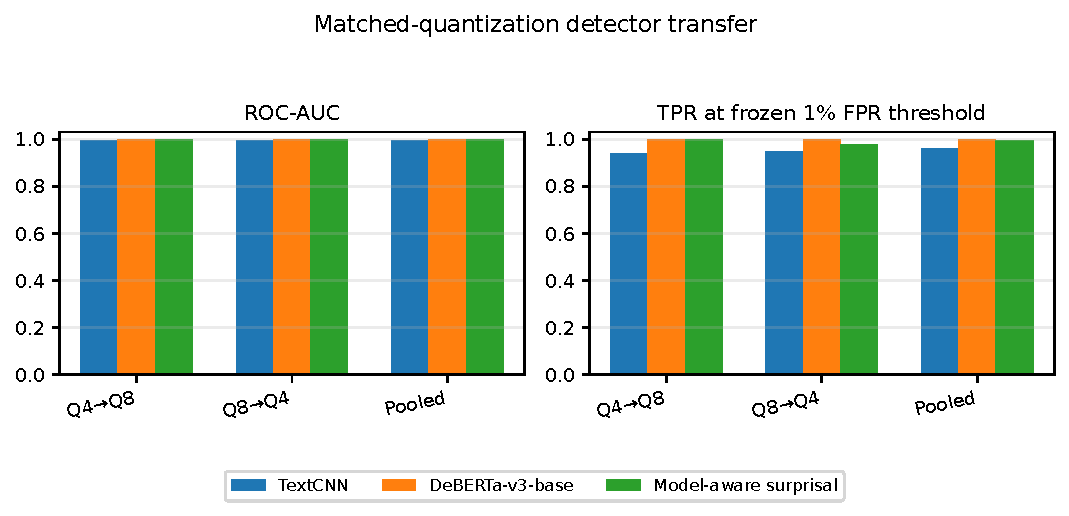
\includegraphics[width=\textwidth]{figures/matched_quantization_detector_transfer.pdf}
\caption{\label{fig:v3-cross-quant-detectors}\textbf{Detector transfer across Q4\_K\_M and Q8\_0.} Detection remains strong in both directions, while observed FPR can exceed the validation target.}
\end{figure}

The analysis isolates two quantizations of one model revision under one inference backend. It does not generalize to other Qwen revisions, architectures, bit widths, quantizers, backends, or hardware. In particular, the data do not justify stating that Q8 is generally more recoverable than Q4.

\section*{Supplementary Note S15: V3 provenance and remaining boundaries}\label{si:s15}

The V3 run manifest binds the detector inputs, model-backed generations, artifact hashes, backend, model and tokenizer identities, partitions, and validation status. The final validation report records \path{status: pass}, exact artifact-manifest path and checksum validation for 5,833 entries, 24 fit-metadata files, 24 prediction files, strict leakage-audit success, conditional entropy-capacity validation, and paired quantization-recovery source validation. The generation-analysis validation records 18/18 calibration traces, 720/720 entropy generations, 1,920/1,920 Q4 replays, 960/960 Q4 visible-recovery records, 1,920/1,920 Q8 generations, and zero failure records. Machine-readable tables and full provenance are retained under \path{results/revision_v3}; the manuscript reports from those sealed outputs rather than rerunning generation.

\begin{longtable}{L{0.23\textwidth}L{0.32\textwidth}L{0.36\textwidth}}
\caption{\label{tab:v3-boundaries}Remaining boundaries after the targeted V3 evaluations.}\\
\toprule
Issue & Added evidence & Boundary that remains \\
\midrule
\endfirsthead
\toprule
Issue & Added evidence & Boundary that remains \\
\midrule
\endhead
Saved-ID replay & Perfect primary and paired-quantization replay under recorded configurations & Requires token IDs, exact model/tokenizer/quantization, rendering, filters, and span boundaries; not ordinary visible-text communication \\
Visible-text transport & 88/144 historical robustness recovery; 732/960 Q4 and 758/960 Q8 in one paired matrix & Paraphrase, markdown/format transfer, cross-model decoding, and retokenization remain fragile or unsuccessful \\
Strict deduplication & Component-safe split with zero declared cross-partition links & Does not detect semantic paraphrases below the 0.95 character-\(n\)-gram threshold \\
Human-authored controls & 250 frozen Dolly negatives across 16 templates & Not a participant study; sparse genre coverage and generic machine/human signal remain \\
Unseen families & Three leave-one-family-out tests & Not every architecture, training corpus, model size, proprietary system, or decoding stack \\
Adaptive detection & Two data-adaptive text-only detectors and an exact-model-aware likelihood attacker & Strong but not exhaustive attackers or deployment distributions \\
Low-FPR reporting & Exact counts and validation-frozen thresholds; matched 0.1\% estimates where supported & Human, family, entropy, and quantization tests have fewer than 1,000 negatives and no empirical 0.1\% resolution \\
Entropy gating & 120 attempts per gate; capacity, length, recovery, quality, and detector outcomes & Two templates; thresholds from 768 positions/model; strict capacity conditional on 114 completions; exact-model AUC remains 0.9904 \\
Quantization & Paired Q4\_K\_M/Q8\_0 recovery and bidirectional detector transfer & One pinned Qwen revision, two quantizations, one backend; no supported general Q8 advantage \\
Naturalness & Automated surface/model diagnostics and a human-authored control corpus & No participants or human ratings; controls are not evidence of human-perceived naturalness \\
Deployment/security & Failure surfaces and strong adverse detectability are documented & No real-world deployment, robust channel, secrecy proof, cryptographic protection, or undetectability \\
\bottomrule
\end{longtable}

The bounded evaluations directly address the requested controls, leakage prevention, held-family transfer, adaptive and model-aware attackers, low-FPR reporting, entropy gating, and quantization sensitivity. They narrow and refine the empirical claim. They do not convert RankCloak into an undetectable, robust, secure, deployable, or practical covert channel.

\bibliography{references}

\end{document}
